\documentclass{IEEEcsmag}

\usepackage[colorlinks,urlcolor=blue,linkcolor=blue,citecolor=blue]{hyperref}

\usepackage{graphicx}
\usepackage[font=small]{subcaption}
\usepackage[english]{babel}
\usepackage{multirow} 
\usepackage{comment}
\usepackage{amssymb}
\usepackage[super,sort,compress]{cite}

\expandafter\def\expandafter\UrlBreaks\expandafter{\UrlBreaks\do\/\do\*\do\-\do\~\do\'\do\"\do\-}
\usepackage{upmath,color}


\jvol{XX}
\jnum{XX}
\paper{8}
\jmonth{Month}
\jname{Publication Name}
\jtitle{Publication Title}
\pubyear{2021}

\newtheorem{theorem}{Theorem}
\newtheorem{lemma}{Lemma}


\setcounter{secnumdepth}{0}

\begin{document}

\sptitle{Article Type: Description  (see below for more detail)}

\title{Face reconstruction guided by forensic sketches}

\author{Edson Odake}
\affil{Federal University of Paraná, Curitiba, Paraná, 81530-000, Brazil}

\author{Eduardo P. Ribeiro}
\affil{Federal University of Paraná, Curitiba, Paraná, 81530-000, Brazil}

\markboth{THEME/FEATURE/DEPARTMENT}{THEME/FEATURE/DEPARTMENT}

\begin{abstract}\looseness-1Forensic sketching translates a victim's description into a visual representation of the suspect but often lacks detail for reliable identification. This paper proposes a Conditional Variational Autoencoder (CVAE) to generate photorealistic faces from forensic sketches without requiring paired sketch-photo datasets. The model enables interactive generation with interpretable attributes and is evaluated on multiple databases. Compared to simpler methods, it produces images that are 56.8\% more similar to the suspect's original photo based on a Facenet metric. The generated images were also used to identify hypothetical suspects from a small database, demonstrating its practical applicability in law enforcement.
\end{abstract}

\maketitle

\chapteri{T}ransforming insights into a concrete idea is a recurrent skill in any creative field. It has been considered a uniquely human capability, as machines can't replicate this process. However, this notion is changing with AI tools that assist creative processes. Software engineers often use Large Language Models (LLMs) to find technical solutions for problems more quickly. Beyond technical applications, these tools are utilized for marketing strategies, content creation, and exploring new research directions \cite{10.1145/3613904.3642698}, encouraging a collaborative interaction between humans and AI.

In forensic investigations, a model trained to reconstruct a facial photo based on sketches could be useful for suspect identification and recognition. Since sketches dismiss color information, additional inputs could be provided to inform more specific characteristics. Forensic artists create facial sketches based on witness descriptions. These sketches could be fed into the model to produce a more realistic image, helping capture public attention and potentially generating tips for identifying suspects. These images could also be integrated with digital technologies for recognizing a suspect against a database \cite{devakumar_forensic_2023}.

Despite advances in generative algorithms, the methods currently used to create faithful facial representations from sketches usually depend on limited databases that pair sketches with original photos \cite{10466756, bushra2021}, a practice that reduces scalability and restricts style diversity. Furthermore, models trained on unpaired images are only evaluated on artificial or digital sketches \cite{li2020}. This evaluation fails to account for hand-drawn faces, limiting the performance on more traditional sketching forms. The literature also lacks a systematic estimation of how faithfully the generated facial features resemble the original.

This paper presents a generative model that transforms facial sketches into photorealistic images. Unlike common approaches, the model employs a stochastic edge map extraction method to improve generalizability. A novel architecture is introduced combining a Conditional Variational Autoencoder (CVAE) with skip connections \cite{he2016} and attention mechanisms \cite{oktay2022} to improve image quality. The model is trained without relying on paired images, disregarding the need to create an extensive sketch database, and two scenarios are built to evaluate the model on recognition and identification tasks.

The paper is structured as follows: It begins by explaining challenges in forensic applications and the limitations of existing approaches. Next, it describes the technologies and methods used to develop this application. Then a comparative analysis, evaluating the performance of different models. At last, a conclusion summarizing the findings and discussing directions for future research.


\section{Forensic Application}
\label{sec:related}

\smallskip

The synthesis of pictures guided by sketches is essentially an image-to-image translation problem, which seeks to optimize the mapping between the sketch and the photorealistic domains. The most commonly used models for this task are Variational Autoencoders (VAEs) and Generative Adversarial Networks (GANs) \cite{pang2022}.

Numerous architectures based on GANs and VAEs have been developed to support forensic investigations \cite{bushra2021,sun2022, di2017, junior2024sketch}. However, these models are often trained and evaluated on controlled datasets, which fail to capture the complexity of forensic scenarios. The sketch characteristic varies depending on the artist, requiring extensive evaluation to ensure applicability in forensic science. Additionally, little attention is given to verifying whether the generated images are helpful for suspect identification. 

After developing a model for generating faces, it is important to guarantee that it aligns with the intended application. Two procedures are proposed to check the performance of a generative model in forensic investigations:

\begin{itemize} 
\item Reconstruction: Evaluates the similarity between the original and generated face using pixelwise and perceptual metrics, providing an overall measure of the model's capability of generating a photorealistic representation from sketches.
\item Identification: Determines whether the generated image retains enough features to recognize the suspect. The model is tested by matching the generated image to the correct suspect within a database containing multiple faces.
\end{itemize}

These methods are defined to estimate the model's performance in forensic applications where sketches of varying styles and artistic interpretations are present.

\section{Methodology}
\label{sec:methodology}

\smallskip

\subsection{Preprocessing pipeline}
\label{subsec:pipeline}

A stochastic pipeline is introduced to mimic various sketching styles, enhancing generalization across a wider range of edge map characteristics. It consists of:

\begin{itemize}
    \item Edge detection: Maps drawings and photos to the "edge space". The edge is extracted from the original images using OpenCV Canny detector \cite{canny1986}, adjusting weak and strong thresholds that control the detection sensibility.
    \item  Closing operation: Uses the dilation morphological operation to extend the edges and close gaps, followed by erosion to refine the edges and reduce thickness. This sequence provides a more continuous edge map.
    \item Gaussian blur: Applied to remove noise and add variability in edge width. It's implemented using a Gaussian filter with a stochastic kernel size, which smooths the image by averaging the pixels based on a Gaussian distribution.
    \item Binarization: A threshold is used to standardize the intensity. This process converts the edge map into a binary representation, defining whether a pixel is an edge or not, and disregarding intensity variations.
\end{itemize}

The pipeline parameters are randomly set for each processed image, altering edge sensitivity and thickness.

\subsection{Proposed Architecture}
\label{subsec:architecture}

The proposed architecture is illustrated in figure \ref{fig:cvae architecture}. The model transforms sketches into photorealistic images while enabling fine-tuning through conditional inputs and preprocessing parameters.

Skip connections mitigate the risk of losing structural information as the image is processed through deeper layers, ensuring a more detailed reconstruction \cite{he2016}. These connections bridge the encoder and decoder layers, ensuring that features with higher resolution from the early stages of the network are available during the upsampling process. The attention mechanism is placed before the concatenation of skip connections. The attention cell calculates the relevance of different image parts, and the important areas are emphasized during the reconstruction process \cite{oktay2022}. Residual connections are added to prevent overfitting since unnecessary layers can be skipped, allowing the network to focus on relevant transformations \cite{he2016}.

\begin{figure*}
    \centering
    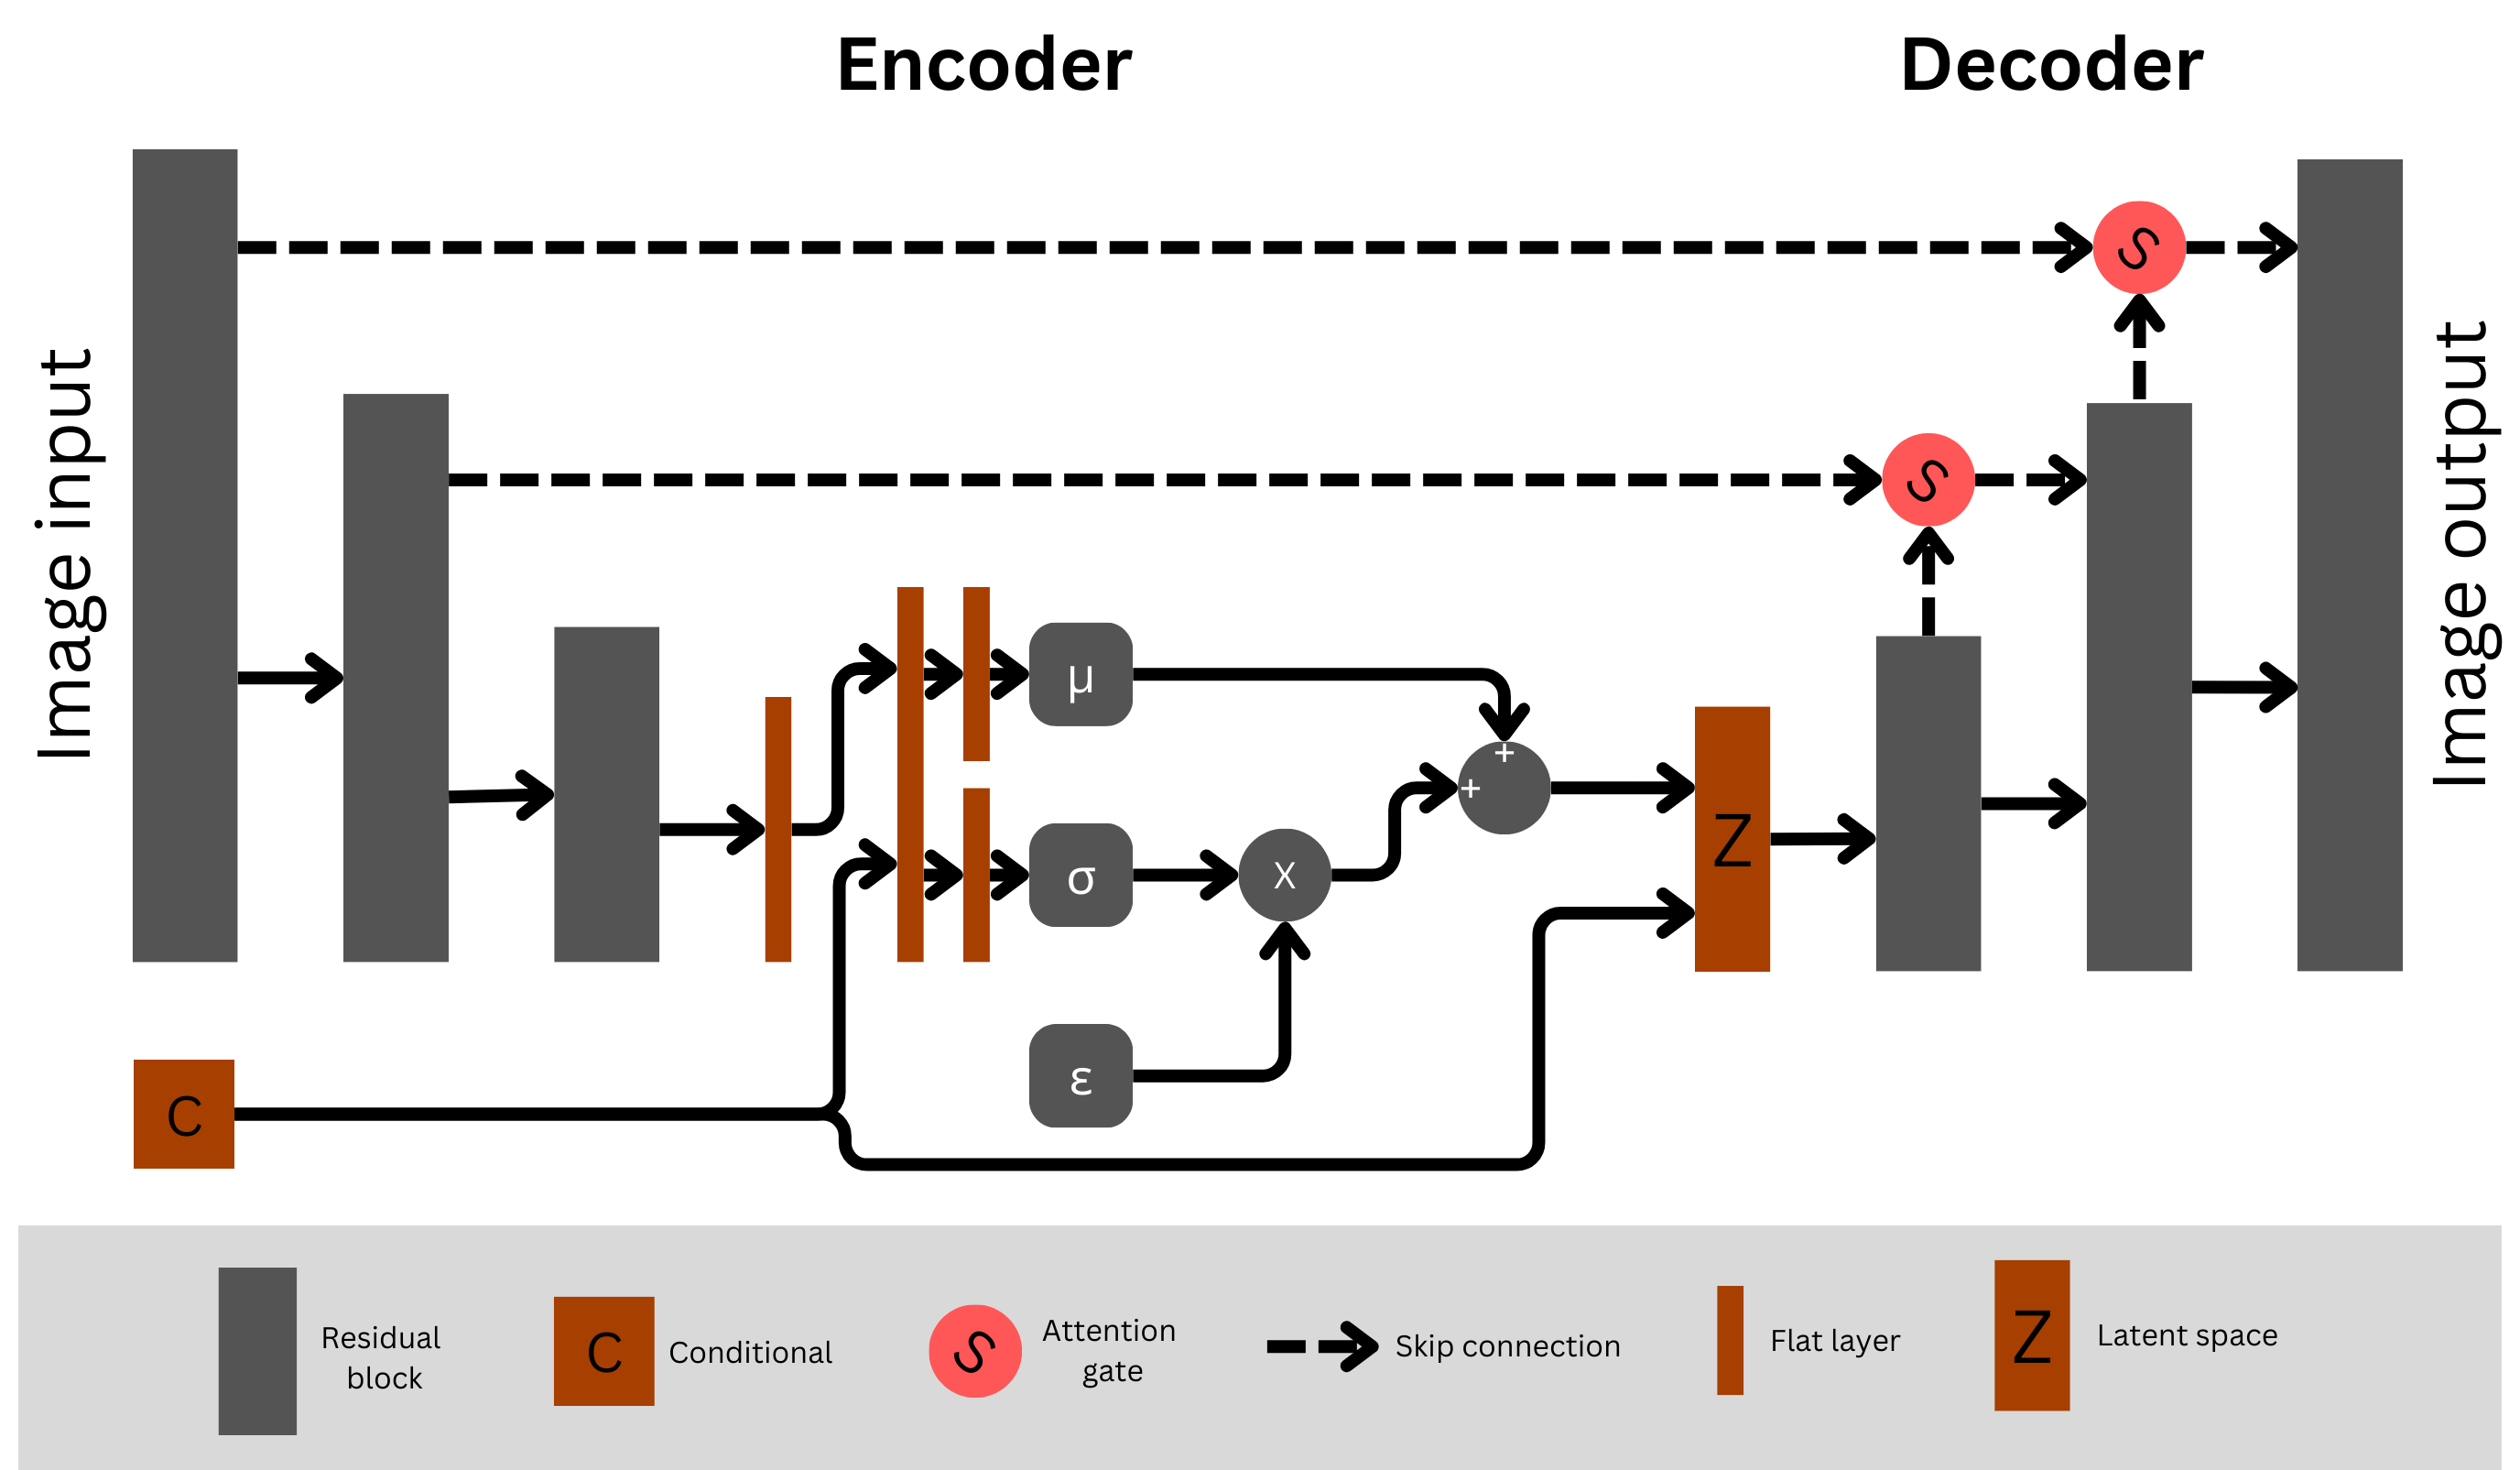
\includegraphics[width=0.8\textwidth]{images/architechture.png}
    \caption{Proposed model architecture.}
    \label{fig:cvae architecture}
\end{figure*}

%\subsection{Objective Function}
%\label{subsec:objective}

The CVAE employs two components (the reconstruction and the regularization term) in its loss function (\(\mathcal{L}\)), as shown in:

\begin{equation}
    \label{eq:loss}
    \begin{split}
    \mathcal{L}  = -\frac{1}{2} \sum_i \left(1 + \log(\sigma_i^2) - \sigma_i^2 - \mu_i^2 \right) \\ - \sum_l \mathbb{E}_{z \sim q_\theta(z|x_i)} \left[ \log p(x_i|z^{(i, l)}) \right]
    \end{split}
\end{equation}

The reconstruction loss is analogous to the vanilla autoencoder (AE): \(- \sum_l \mathbb{E}_{z \sim q_\theta(z|x_i)} \left[ \log p(x_i|z^{(i, l)}) \right]\). Where, \(\mathbb{E}_{z \sim q_\theta(z|x_i)}\) denotes the expectation over the latent variable \(z\), sampled from the approximate posterior distribution \(q_\theta(z|x_i)\), and \(\log p(x_i|z^{(i, l)})\) is the log-likelihood of the data point \(x_i\) given the latent variable \(z^{(i, l)}\).

The regularization term (derived from the KL divergence), \(-\frac{1}{2} \sum_i \left(1 + \log(\sigma_i^2) - \sigma_i^2 - \mu_i^2 \right)\), measures the similarity between two probability distributions, encouraging the encoded data to resemble a Gaussian distribution. It prevents the model from creating an overly complex latent space that doesn't generalize to new data. \(\sigma_i^2\) is the variance, and \(\mu_i\) is the mean of the latent variable distribution for the \(i\)-th data point. Instead of directly sampling from the latent space, the model samples a noise variable \(\varepsilon\) from a normal distribution and reparameterizes the latent variable as: \(z = \mu + \sigma^2 \varepsilon \), without breaking the backpropagation.

The Structural Similarity Index Measure (SSIM) is applied as the reconstruction metric:

\begin{equation}
    \label{eq:ssim}
    \text{SSIM}(x, y) = \frac{(2 \mu_x \mu_y + C_1)(2 \sigma_{xy} + C_2)}{(\mu_x^2 + \mu_y^2 + C_1)(\sigma_x^2 + \sigma_y^2 + C_2)}
\end{equation}

where $\mu_x$ and $\mu_y$ are the mean values of the images $x$ and $y$, $\sigma_x^2$ and $\sigma_y^2$ are the variances, and $\sigma_{xy}$ is the covariance of $x$ and $y$. Constants $C_1$ and $C_2$ are small values included to stabilize the division with weak denominators.

SSIM is a more perceptual evaluation than Mean Squared Error (MSE) or Peak Signal-to-Noise Ratio (PSNR), providing a human-like image similarity measure. SSIM evaluates the similarity between images considering changes in structural information, luminance, and contrast \cite{wang2004}.

A constant value (named $\beta$) is multiplied with the regularization term to modulate its weight in the loss function, balancing the latent space constraint \cite{higgins2022}. When $\beta$ is significantly greater than one, the regularization term dominates, leading to blurrier images since the emphasis on reconstruction diminishes. Conversely, if $\beta$ is close to zero, the influence of the regularization term is reduced, resulting in a less continuous latent space. Choosing an appropriate $\beta$ helps preserve image quality and maintain a well-structured latent space.

\subsection{Training}
\label{subsec:training}

Three distinct models are trained for comparison: a vanilla AE model, a proposed AE architecture enhanced with an attention mechanism and skip connections, and the complete CVAE as proposed. The vanilla AE allows us to establish a performance benchmark and understand its limitations. The proposed AE model possesses attention mechanisms and skip connections, creating more detailed and sharper images than the vanilla AE. The CVAE incorporates conditional inputs for users to interact with and modify the generated image.

Each model consisted of multiple convolutional layers with 3x3 kernel sizes, followed by batch normalization and ReLU activation functions to introduce non-linearity. The vanilla AE architecture included 13 layers. While sharing a similar core structure, the proposed AE and the CVAE architectures included additional layers for residual connections, attention mechanisms, and conditional input processing, bringing the total to 26 layers. These additions primarily serve to improve regularization. All models were trained for 15 epochs with a batch size of 64, using the ADAM optimizer with a learning rate 0.001. Batch normalization was applied after each convolutional layer to mitigate issues like exploding gradients.

The strong threshold of the Canny edge detector was randomly sampled between 100 and 200. The weak threshold was determined by multiplying the strong threshold by a factor sampled from a Gaussian distribution with a mean of 0.5 and a variance of 0.1. Additionally, the size of the Gaussian filter varied randomly between a 3x3 and a 7x7 matrix. These variations resulted in edge maps with different sensitivities and edge widths, enhancing the model's ability to interpret maps with varying levels of detail and noise. The morphological operation used a 3x3 kernel, and the binarization threshold was set at 0.5. An early stopping callback wasn't implemented because the models often ceased training while producing blurry images.

The model is trained without using sketches. During training, each photo is processed through a stochastic pipeline to extract an edge map, and fed into the generative model. The model aims to reconstruct the target image based on the features captured in the edge map (as shown in Figure \ref{fig:trainingEvaluationComparison}).

\begin{figure*}[ht]
    \centering
    \begin{subfigure}{0.36\textwidth}
        \centering
        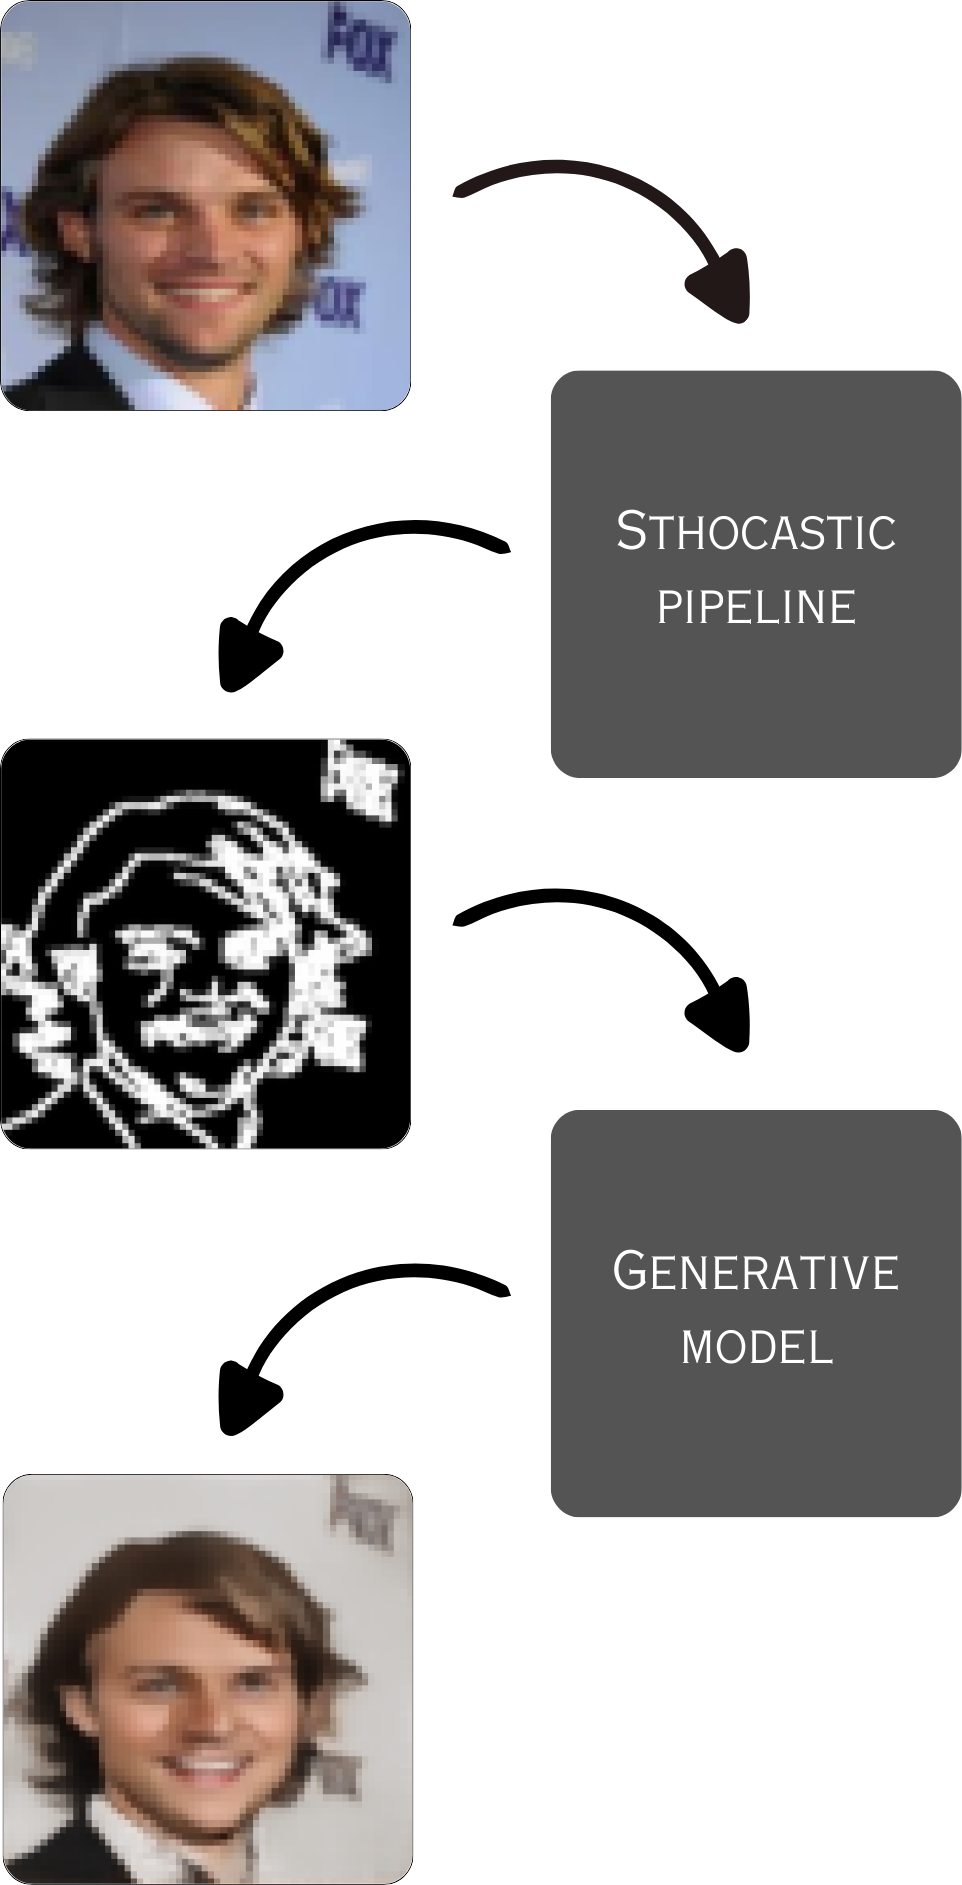
\includegraphics[width=0.72\linewidth]{example image/trainingFramework.png}
        \caption{Training process}
        \label{fig:trainingProcess}
    \end{subfigure}
    \hfill
    \begin{subfigure}{0.36\textwidth}
        \centering
        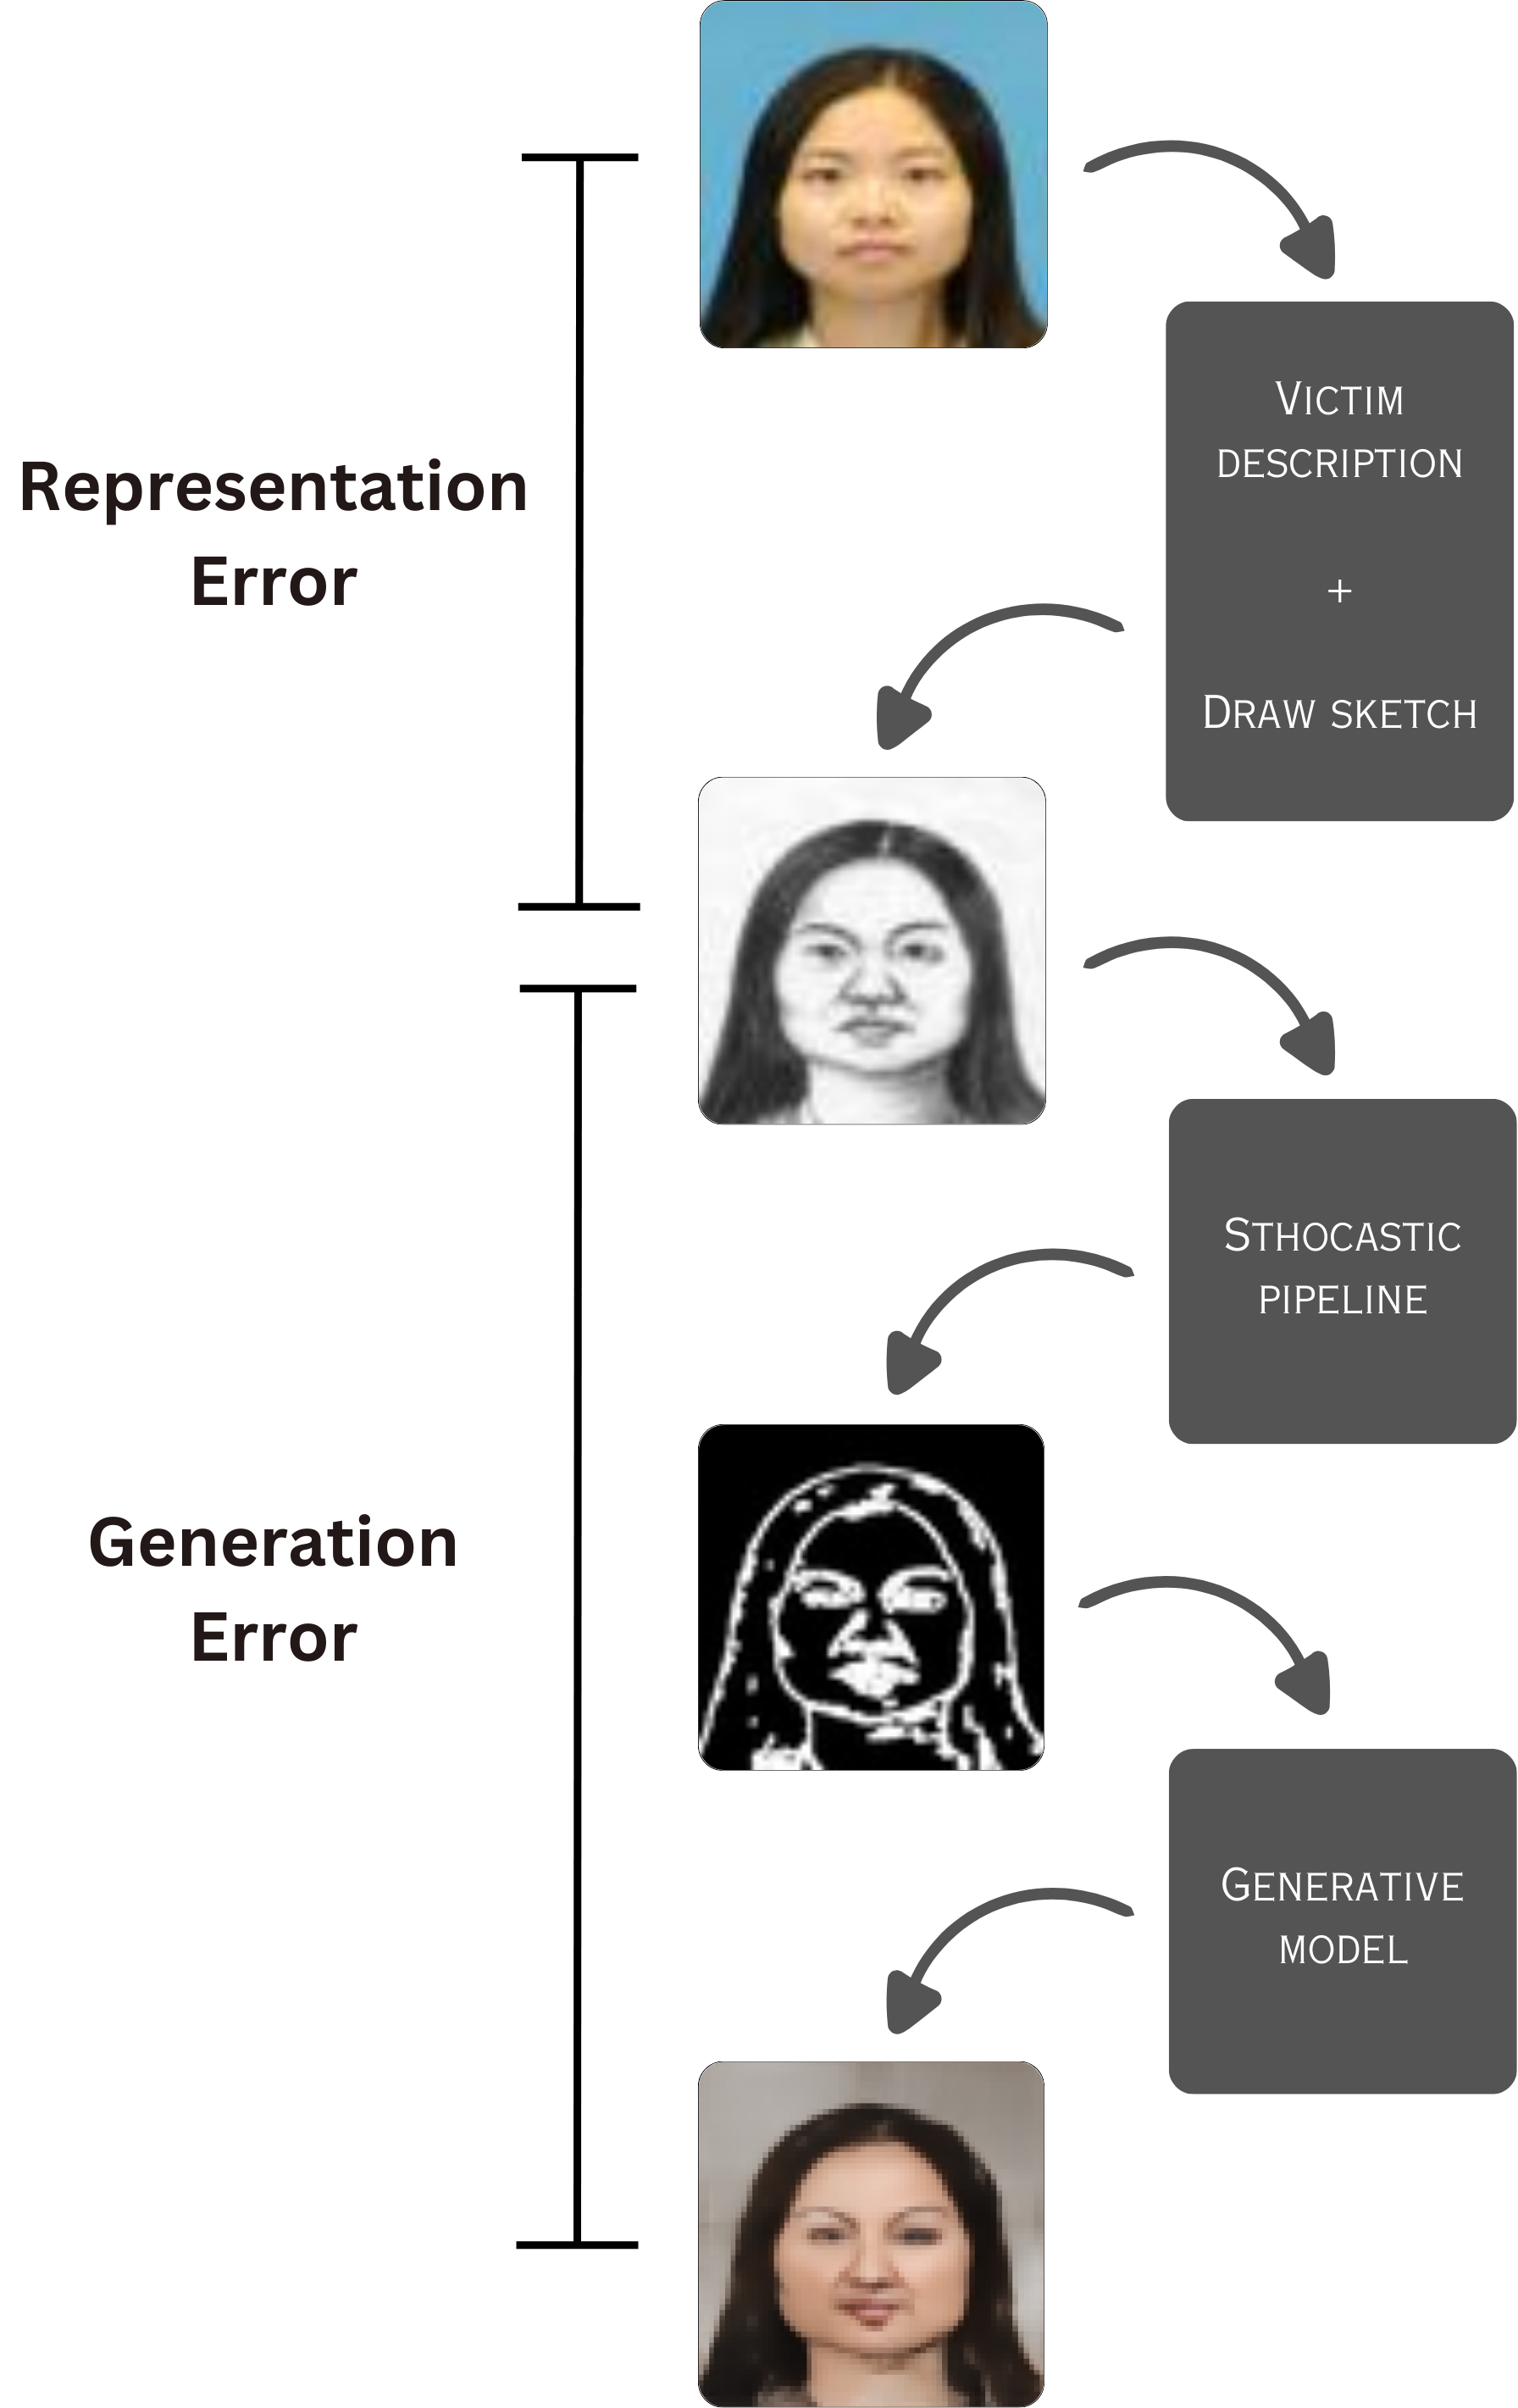
\includegraphics[width=0.95\linewidth]{example image/validationFramework.png}
        \caption{Evaluation process}
        \label{fig:evaluationProcess}
    \end{subfigure}
    \caption{Comparison of the training and evaluation processes.}
    \label{fig:trainingEvaluationComparison}
\end{figure*}


\subsection{Evaluation Metric}
\label{subsec:evaluation}

Four metrics are used to evaluate the generated images: MSE, SSIM \cite{wang2004}, Frechet Inception Distance (FID) Score \cite{dowson_frechet_1982}, and Facenet Euclidean distance \cite{schroff_facenet_2015}. MSE is a pixelwise metric that measures basic reconstruction accuracy. SSIM, on the other hand, captures perceptual features by evaluating luminance, contrast, and structural information. The FID Score uses a pre-trained network to identify image patterns, providing a higher-level analysis. Let \(\mu_r\) and \(\Sigma_r\) be the mean and covariance activations of the real images, while \(\mu_g\) and \(\Sigma_g\) are related to the generated images (these variables represent high-level features from the Inception V3 model). The FID is defined as \cite{dowson_frechet_1982}:
\begin{equation}
    \label{eq:FID}
    \text{FID} = \| \mu_r - \mu_g \|^2 + \text{Tr}(\Sigma_r + \Sigma_g - 2 (\Sigma_r \Sigma_g)^{\frac{1}{2}})
\end{equation}

where:
\begin{itemize}
  \item \(\| \mu_r - \mu_g \|^2\) is the squared Euclidean output distance between the means of the real and generated images after passing the model.
  \item \(\text{Tr}\) denotes the trace of a matrix (sum of its diagonal elements).
  \item \(\Sigma_r\) and \(\Sigma_g\) are the covariance matrices of the activations for the real and generated images, respectively.
\end{itemize}

Facenet is a pre-trained deep-learning model developed for face recognition, verification, and clustering. It's trained with the Triplet loss and uses a deep convolutional network to map images of faces into a compact Euclidean space where distances directly correspond to a measure of face similarity \cite{schroff_facenet_2015}. Facenet captures the nuances of facial similarity, which is essential for applications in forensic contexts.

Unlike in training, the evaluation process uses a sketch to generate the image, as shown in figure \ref{fig:trainingEvaluationComparison}, which includes the additional step of drawing the facial sketch. The drawing is passed through the edge extraction pipeline, and the resulting edge map is fed into the generative model. Manually drawing the sketch introduces a Representation Error. Therefore, the total evaluation error is the sum of this Representation Error and the Generation Error.

\subsection{Databases}
\label{subsec:databases}

The models are trained using the CelebA database \cite{liu2015}, which comprises over 202,599 images with dimensions of 178x218 pixels. Each image is annotated with a binary vector of 40 attributes. For this study, 14 attributes are selected and filtered to serve as conditional inputs for the CVAE. These attributes are chosen based on their relevance and ability to complement the sketch information. 

Since the CelebA database contains no sketches, the evaluation is extended using different sketch databases. One is the CUHK student database \cite{zhang_coupled_2011}, which provides pairs of sketches and original pictures of young Asian individuals. This database doesn't have the 40 attributes available in CelebA and was manually annotated for each image.

Random digitally drawn images were collected from the internet to extend the evaluation. Unlike the other databases, these images don't have matching pairs of original photos and sketches. As a result, the scope of this evaluation is limited to a more subjective analysis, which helps to understand how well the model performs with digitally drawn sketches.

\section{Results}
\label{sec:results}

\subsection{Reconstruction quality}
\label{subsec:reconstructionQuality}

To assess whether the generated image can reproduce the characteristics of the original face, the outputs of the three models are compared: a vanilla AE, the proposed AE, and the CVAE. Figure \ref{fig:CombinedComparison} presents the original images, their sketch representations, and the corresponding generated images from the CelebA and the CUHK student database.

\begin{figure*}[ht]
\setcounter{subfigure}{0}
    \centering
    % Row 1 - Original
    \begin{subfigure}{0.12\textwidth}
        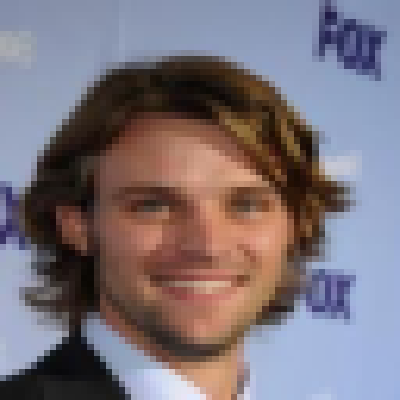
\includegraphics[width=\linewidth]{images/CelebA/1/original_4.png}
        %\caption{CelebA 1}
    \end{subfigure}
    \begin{subfigure}{0.12\textwidth}
        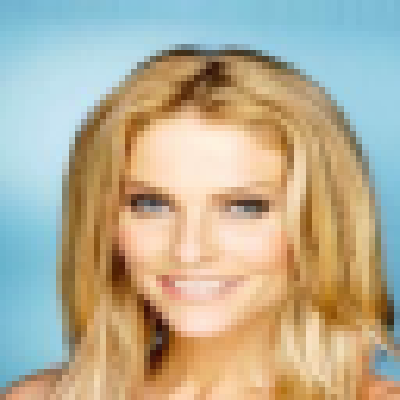
\includegraphics[width=\linewidth]{images/CelebA/1/original_2.png}
        %\caption{CelebA 2}
    \end{subfigure}
    \begin{subfigure}{0.12\textwidth}
        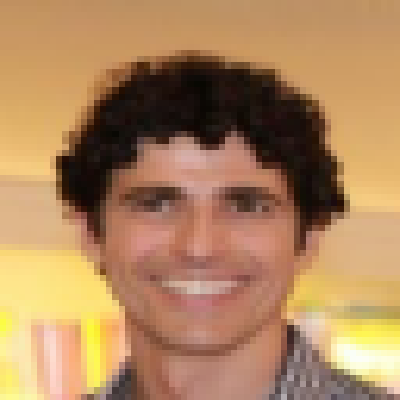
\includegraphics[width=\linewidth]{images/CelebA/1/original_5.png}
        %\caption{CelebA 3}
    \end{subfigure}
    \begin{subfigure}{0.12\textwidth}
        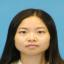
\includegraphics[width=\linewidth]{CUHK_Student/original_resized/f1-001-01-sz1.jpg}
        %\caption{CUHK 4}
    \end{subfigure}
    \begin{subfigure}{0.12\textwidth}
        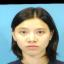
\includegraphics[width=\linewidth]{CUHK_Student/original_resized/f1-008-01-sz1.jpg}
        %\caption{CUHK 5}
    \end{subfigure}
    \begin{subfigure}{0.12\textwidth}
        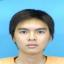
\includegraphics[width=\linewidth]{CUHK_Student/original_resized/M2-018-01-sz1.jpg}
        %\caption{CUHK 6}
    \end{subfigure}

    \smallskip
    \setcounter{subfigure}{0}
    
    % Row 2 - Sketch/Edge Map
    \begin{subfigure}{0.12\textwidth}
        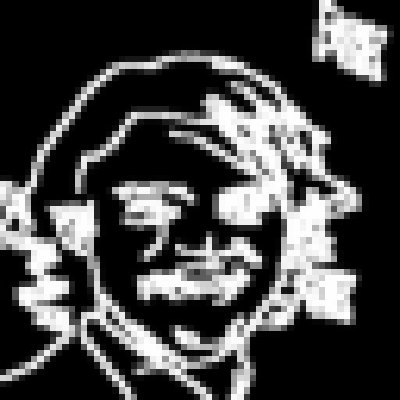
\includegraphics[width=\linewidth]{images/CelebA/1/distorted_4.png}
        %\caption{Edges 1}
    \end{subfigure}
    \begin{subfigure}{0.12\textwidth}
        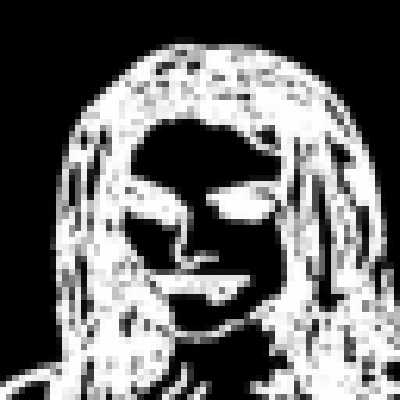
\includegraphics[width=\linewidth]{images/CelebA/1/distorted_2.png}
        %\caption{Edges 2}
    \end{subfigure}
    \begin{subfigure}{0.12\textwidth}
        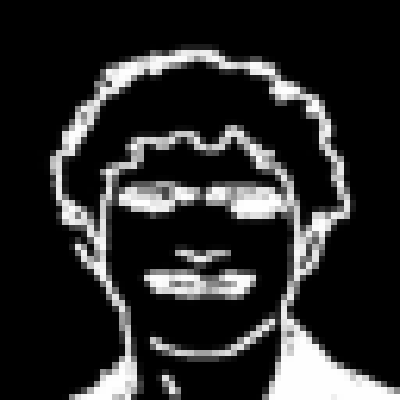
\includegraphics[width=\linewidth]{images/CelebA/1/distorted_5.png}
        %\caption{Edges 3}
    \end{subfigure}
    \begin{subfigure}{0.12\textwidth}
        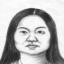
\includegraphics[width=\linewidth]{CUHK_Student/draws_resized/f1-001-01-sz1.jpg}
        %\caption{Sketch 4}
    \end{subfigure}
    \begin{subfigure}{0.12\textwidth}
        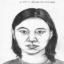
\includegraphics[width=\linewidth]{CUHK_Student/draws_resized/f1-008-01-sz1.jpg}
        %\caption{Sketch 5}
    \end{subfigure}
    \begin{subfigure}{0.12\textwidth}
        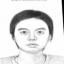
\includegraphics[width=\linewidth]{CUHK_Student/draws_resized/M2-018-01-sz1.jpg}
        %\caption{Sketch 6}
    \end{subfigure}

    \smallskip
    \setcounter{subfigure}{0}

    % Row 3 - Simple AE
    \begin{subfigure}{0.12\textwidth}
        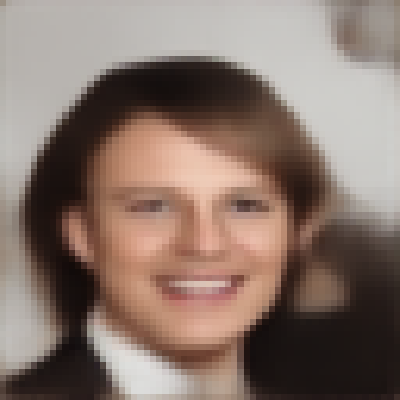
\includegraphics[width=\linewidth]{images/CelebA/1/simple_ae_4.png}
        %\caption{Simple AE 1}
    \end{subfigure}
    \begin{subfigure}{0.12\textwidth}
        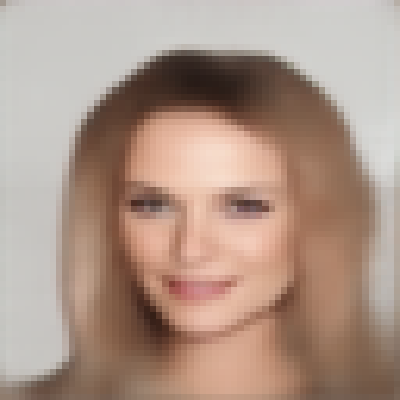
\includegraphics[width=\linewidth]{images/CelebA/1/simple_ae_2.png}
        %\caption{Simple AE 2}
    \end{subfigure}
    \begin{subfigure}{0.12\textwidth}
        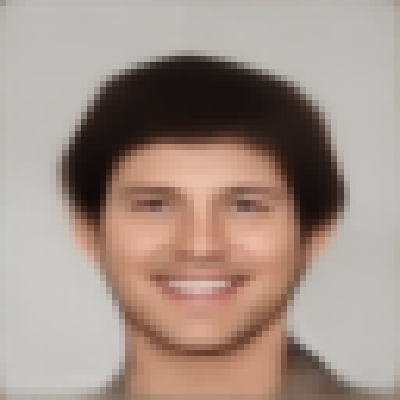
\includegraphics[width=\linewidth]{images/CelebA/1/simple_ae_5.png}
        %\caption{Simple AE 3}
    \end{subfigure}
    \begin{subfigure}{0.12\textwidth}
        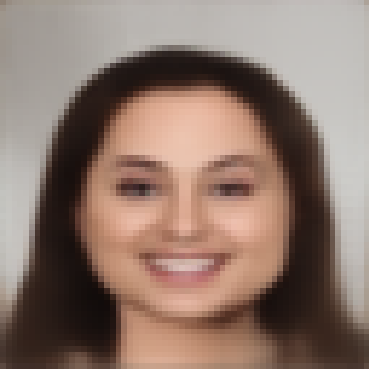
\includegraphics[width=\linewidth]{CUHK_Student/generated_images/f1-001-01-sz1.jpg_AE.png}
        %\caption{Simple AE 4}
    \end{subfigure}
    \begin{subfigure}{0.12\textwidth}
        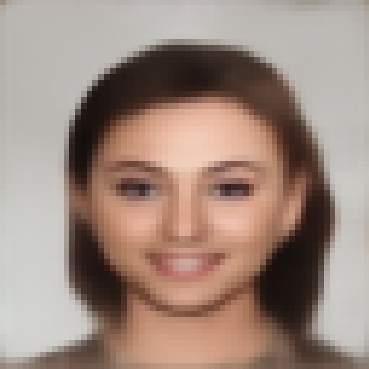
\includegraphics[width=\linewidth]{CUHK_Student/generated_images/f1-008-01-sz1.jpg_AE.png}
        %\caption{Simple AE 5}
    \end{subfigure}
    \begin{subfigure}{0.12\textwidth}
        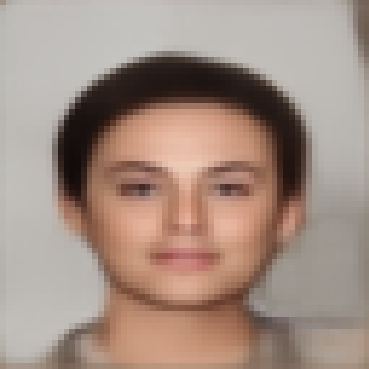
\includegraphics[width=\linewidth]{CUHK_Student/generated_images/M2-018-01-sz1.jpg_AE.png}
        %\caption{Simple AE 6}
    \end{subfigure}

    \smallskip
    \setcounter{subfigure}{0}

    % Row 4 - Proposed AE
    \begin{subfigure}{0.12\textwidth}
        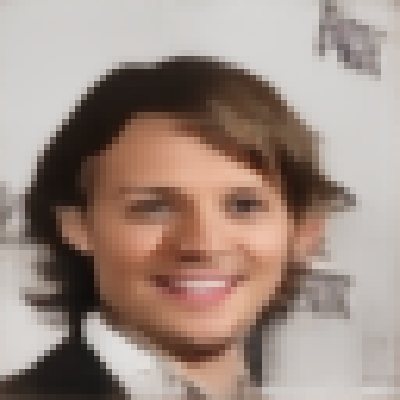
\includegraphics[width=\linewidth]{images/CelebA/1/proposed_ae_4.png}
        %\caption{Prop. AE 1}
    \end{subfigure}
    \begin{subfigure}{0.12\textwidth}
        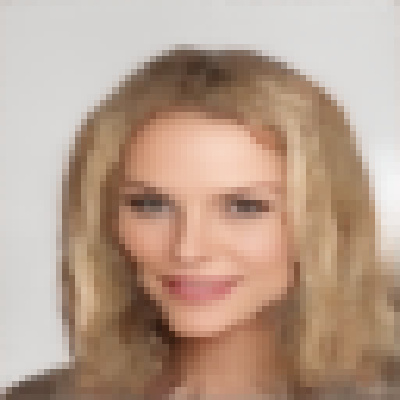
\includegraphics[width=\linewidth]{images/CelebA/1/proposed_ae_2.png}
        %\caption{Prop. AE 2}
    \end{subfigure}
    \begin{subfigure}{0.12\textwidth}
        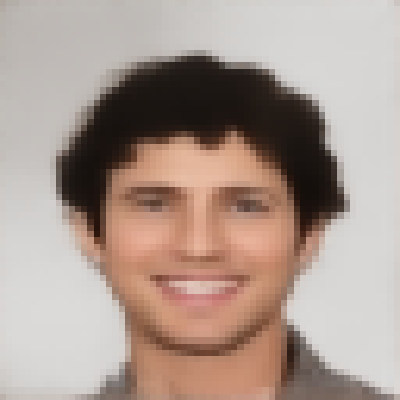
\includegraphics[width=\linewidth]{images/CelebA/1/proposed_ae_5.png}
        %\caption{Prop. AE 3}
    \end{subfigure}
    \begin{subfigure}{0.12\textwidth}
        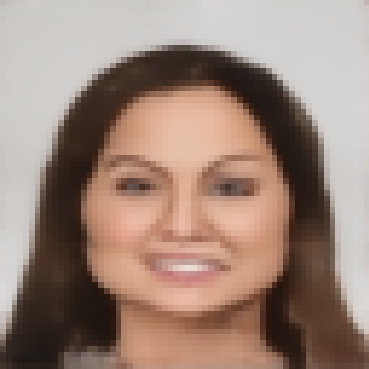
\includegraphics[width=\linewidth]{CUHK_Student/generated_images/f1-001-01-sz1.jpg_AE_UNET.png}
        %\caption{Prop. AE 4}
    \end{subfigure}
    \begin{subfigure}{0.12\textwidth}
        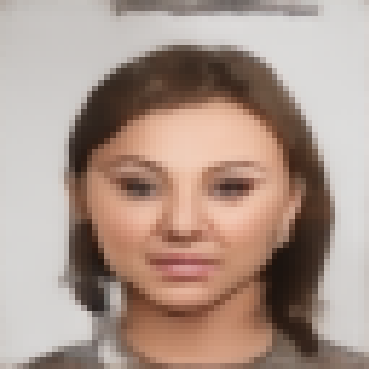
\includegraphics[width=\linewidth]{CUHK_Student/generated_images/f1-008-01-sz1.jpg_AE_UNET.png}
        %\caption{Prop. AE 5}
    \end{subfigure}
    \begin{subfigure}{0.12\textwidth}
        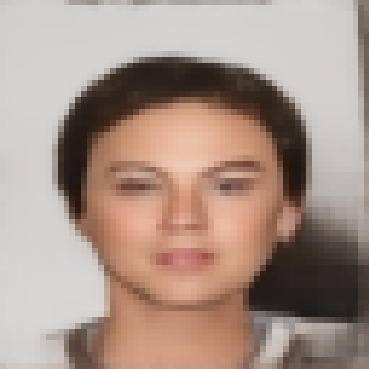
\includegraphics[width=\linewidth]{CUHK_Student/generated_images/M2-018-01-sz1.jpg_AE_UNET.png}
        %\caption{Prop. AE 6}
    \end{subfigure}
    
    \smallskip
    \setcounter{subfigure}{0}

    % Row 5 - Proposed CVAE
    \begin{subfigure}{0.12\textwidth}
        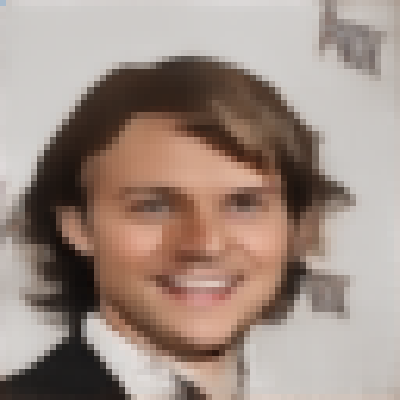
\includegraphics[width=\linewidth]{images/CelebA/1/cvae_4.png}
        %\caption{Prop. CVAE 1}
    \end{subfigure}
    \begin{subfigure}{0.12\textwidth}
        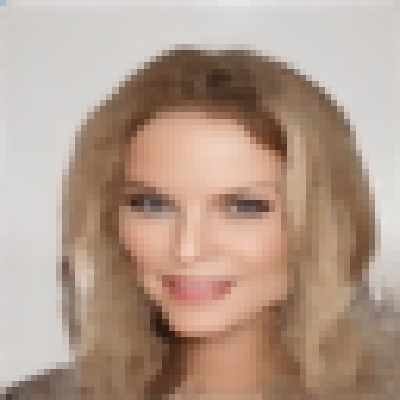
\includegraphics[width=\linewidth]{images/CelebA/1/cvae_2.png}
        %\caption{Prop. CVAE 2}
    \end{subfigure}
    \begin{subfigure}{0.12\textwidth}
        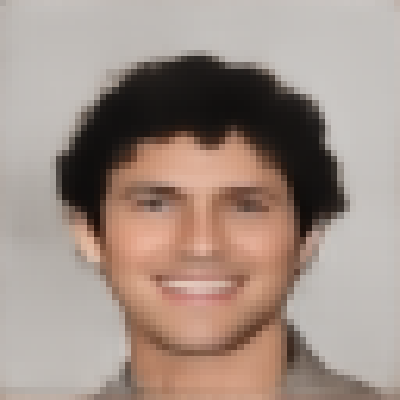
\includegraphics[width=\linewidth]{images/CelebA/1/cvae_5.png}
        %\caption{Prop. CVAE 3}
    \end{subfigure}
    \begin{subfigure}{0.12\textwidth}
        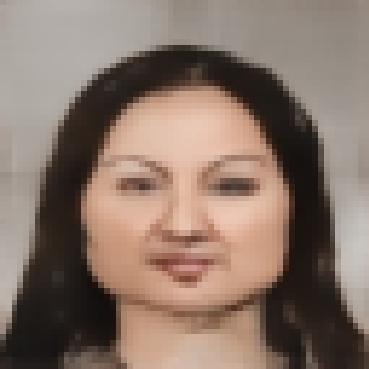
\includegraphics[width=\linewidth]{CUHK_Student/generated_images/f1-001-01-sz1.jpg_CVAE.png}
        %\caption{Prop. CVAE 4}
    \end{subfigure}
    \begin{subfigure}{0.12\textwidth}
        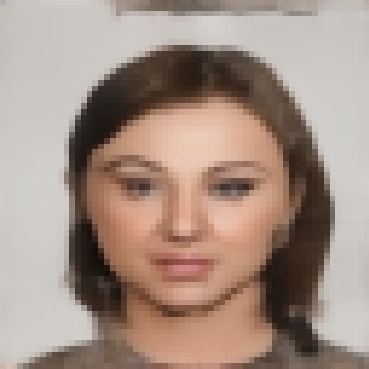
\includegraphics[width=\linewidth]{CUHK_Student/generated_images/f1-008-01-sz1.jpg_CVAE.png}
        %\caption{Prop. CVAE 5}
    \end{subfigure}
    \begin{subfigure}{0.12\textwidth}
        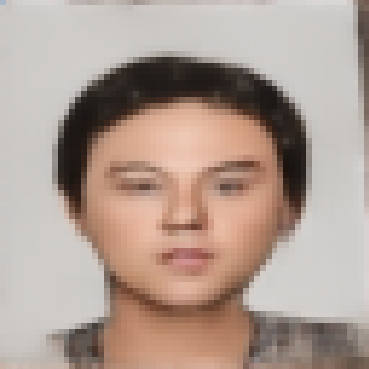
\includegraphics[width=\linewidth]{CUHK_Student/generated_images/M2-018-01-sz1.jpg_CVAE.png}
        %\caption{Prop. CVAE 6}
    \end{subfigure}

    \caption{Comparison of CelebA and CUHK datasets. Columns 1-3: CelebA dataset; Columns 4-6: CUHK dataset. Row 1: Original images; Row 2: Sketch or edge map; Row 3: Vanilla AE; Row 4: Proposed AE; Row 5: CVAE}
    \label{fig:CombinedComparison}
\end{figure*}

The images generated from the vanilla AE are blurrier and more generic than the others. This difference in quality is evident in both subjective visual assessments and perceptual objective metrics (less evident in pixelwise metrics). The proposed AE and the CVAE produced more detailed images. While both proposed models yield similar results, the CVAE performs slightly better. The images generated from the CUHK sketches also demonstrated similar representations of the original faces. These images are generated from a sketch. If the sketch fails to represent some feature, the model will also capture this misinformation when generating the face.

In Figure \ref{fig:ComparisonBar} the quantitative comparison of original and generated CelebA images is observed. Also, Table \ref{tab:similarity} presents the metrics without scale applied. The SSIM metric is inverted (1 - SSIM), meaning smaller SSIM values indicate better results. 

The MSE results were similar across all models, with the proposed CVAE performing slightly better. However, the proposed models outperformed the vanilla AE in SSIM and FID metrics, indicating better preservation of structural and perceptual details in the generated images. Additionally, the CVAE demonstrated a 29.2\% increase in facial similarity when measured with Facenet. As the metrics become more specific, the performance gap between the models also increases.

\begin{figure}[ht]
    \centering
    \begin{subfigure}{0.48\textwidth}
        \centering
        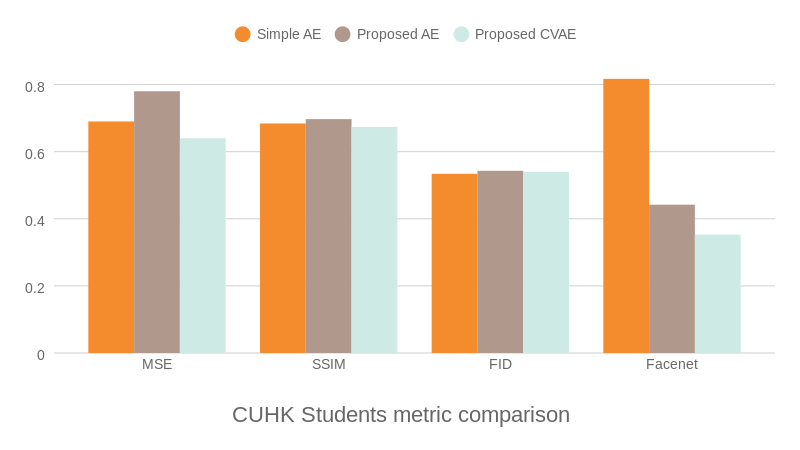
\includegraphics[width=\linewidth]{images/CUHK_Student/3/mse_ssim_comparison.png}
        %\caption{CUHK performance metric comparison.}
        \label{fig:CUHKComparisonBar}
    \end{subfigure}
    \hfill
    \begin{subfigure}{0.48\textwidth}
        \centering
        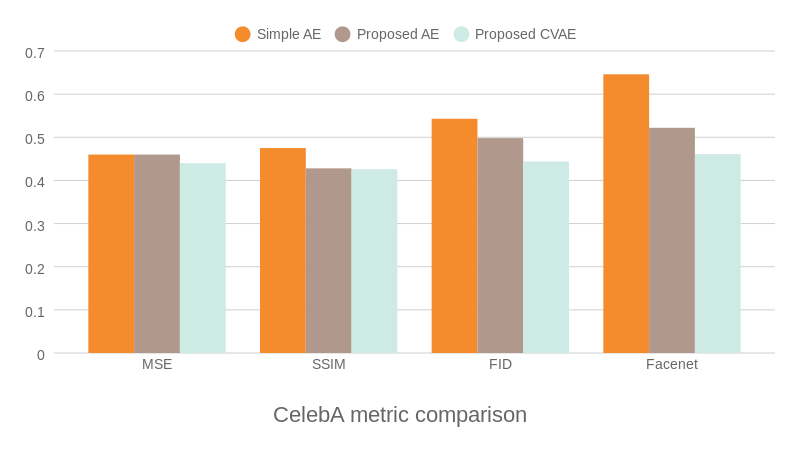
\includegraphics[width=\linewidth]{images/CelebA/3/mse_ssim_comparison.png}
        %\caption{CelebA performance metric comparison.}
        \label{fig:CelebAComparisonBar}
    \end{subfigure}
    
    \caption{Performance metric comparison for CUHK and CelebA datasets on ten samples (Metrics were scaled to the same perspective for illustration purposes).}
    \label{fig:ComparisonBar}
\end{figure}

\begin{table*}
\vspace*{4pt}
\caption{Performance metrics for CelebA and CUHK datasets}
\label{tab:similarity}
\tablefont
\begin{tabular*}{\textwidth}{@{}l p{40pt}<{\raggedright} p{40pt}<{\centering} p{40pt}<{\centering} p{40pt}<{\centering} p{40pt}<{\centering} p{40pt}<{\centering}@{}}
\toprule
\textbf{Model} & 
\textbf{Dataset} & 
\textbf{MSE} & 
\textbf{SSIM} & 
\textbf{PSNR} & 
\textbf{FID} & 
\textbf{Facenet} \\
\colrule
\multirow{2}{*}{Vanilla AE} 
& CelebA & 0.05 & 0.52 & 14.24 & 180.58 & 0.65 \\[3pt]
& CUHK   & 0.07 & 0.32 & 11.69 & 176.18 & 0.82 \\[3pt]
%& CelebA & 0.05 & 0.52 & 180.58 & 0.65 \\[3pt]
%& CUHK   & 0.07 & 0.32 & 176.18 & 0.82 \\[3pt]
\colrule
\multirow{2}{*}{Proposed AE}
& CelebA & 0.05 & 0.57 & 14.51 & 165.54 & 0.52 \\[3pt]
& CUHK   & 0.08 & 0.30 & 11.22 & 180.64 & 0.44 \\[3pt]
%& CelebA & 0.05 & 0.57 & 165.54 & 0.52 \\[3pt]
%& CUHK   & 0.08 & 0.30 & 180.64 & 0.44 \\[3pt]
\colrule
\multirow{2}{*}{Proposed CVAE} 
& CelebA & 0.04 & 0.57 & 14.69 & 147.91 & 0.46 \\[3pt]
& CUHK   & 0.06 & 0.33 & 12.01 & 180.46 & 0.35 \\[3pt]
%& CelebA & 0.04 & 0.57 & 147.91 & 0.46 \\[3pt]
%& CUHK   & 0.06 & 0.33 & 180.46 & 0.35 \\[3pt]
\botrule
\end{tabular*}
\vspace*{8pt}
\end{table*}

In figure \ref{fig:ComparisonBar} a similar comparison is performed using CUHK database. The results show that the more generic metrics (MSE, SSIM, and FID) presented similar results across the different models. The most significant difference is observed with the Facenet-based metric. The vanilla AE displayed a big discrepancy on this metric, indicating that its generated images were less accurate in capturing the essential facial features necessary for recognition. The proposed AE achieved a 53\% improvement compared to the vanilla AE. Meanwhile, the CVAE demonstrated the best performance, with a similarity score that was 56.8\% higher than that of the vanilla AE. Since Facenet is specifically designed for face recognition, achieving good results with this metric indicates the model's ability to generate realistic and recognizable facial images. 

\subsection{Identification quality}
\label{subsec:identificationQuality}

A small sample of random images is selected, including the suspect's face. The sketch is then used to generate a face, which is compared with each individual in the database by calculating the FaceNet Euclidean distance. The similarity of the original suspect is ranked. Rank one indicates the closest match, rank two indicates the second-best match, and so on.

Anil K. Jain emphasized the relevance of database size in evaluating face recognition methods \cite{Jain}. The database size (suspect list) is iterated from five to fifty images, and the metrics are calculated based on this list. The face of each suspect is added to the suspect list and compared with the generated image. The suspect is then removed from the database, and the process is repeated for the next suspect. In the CelebA database, 30 suspects are used, while in the CUHK database, 13 suspects are considered. Figure \ref{fig:accuracy_celeba} shows the accuracy score versus the number of images in the database. The proposed AE achieved the best results, correctly matching 53\% of suspects. The CVAE followed with 50\% accuracy, while the vanilla AE presented the lowest performance at 30\%.

\begin{figure*}[ht]
    \centering
    \begin{subfigure}{0.4\textwidth}
        \centering
        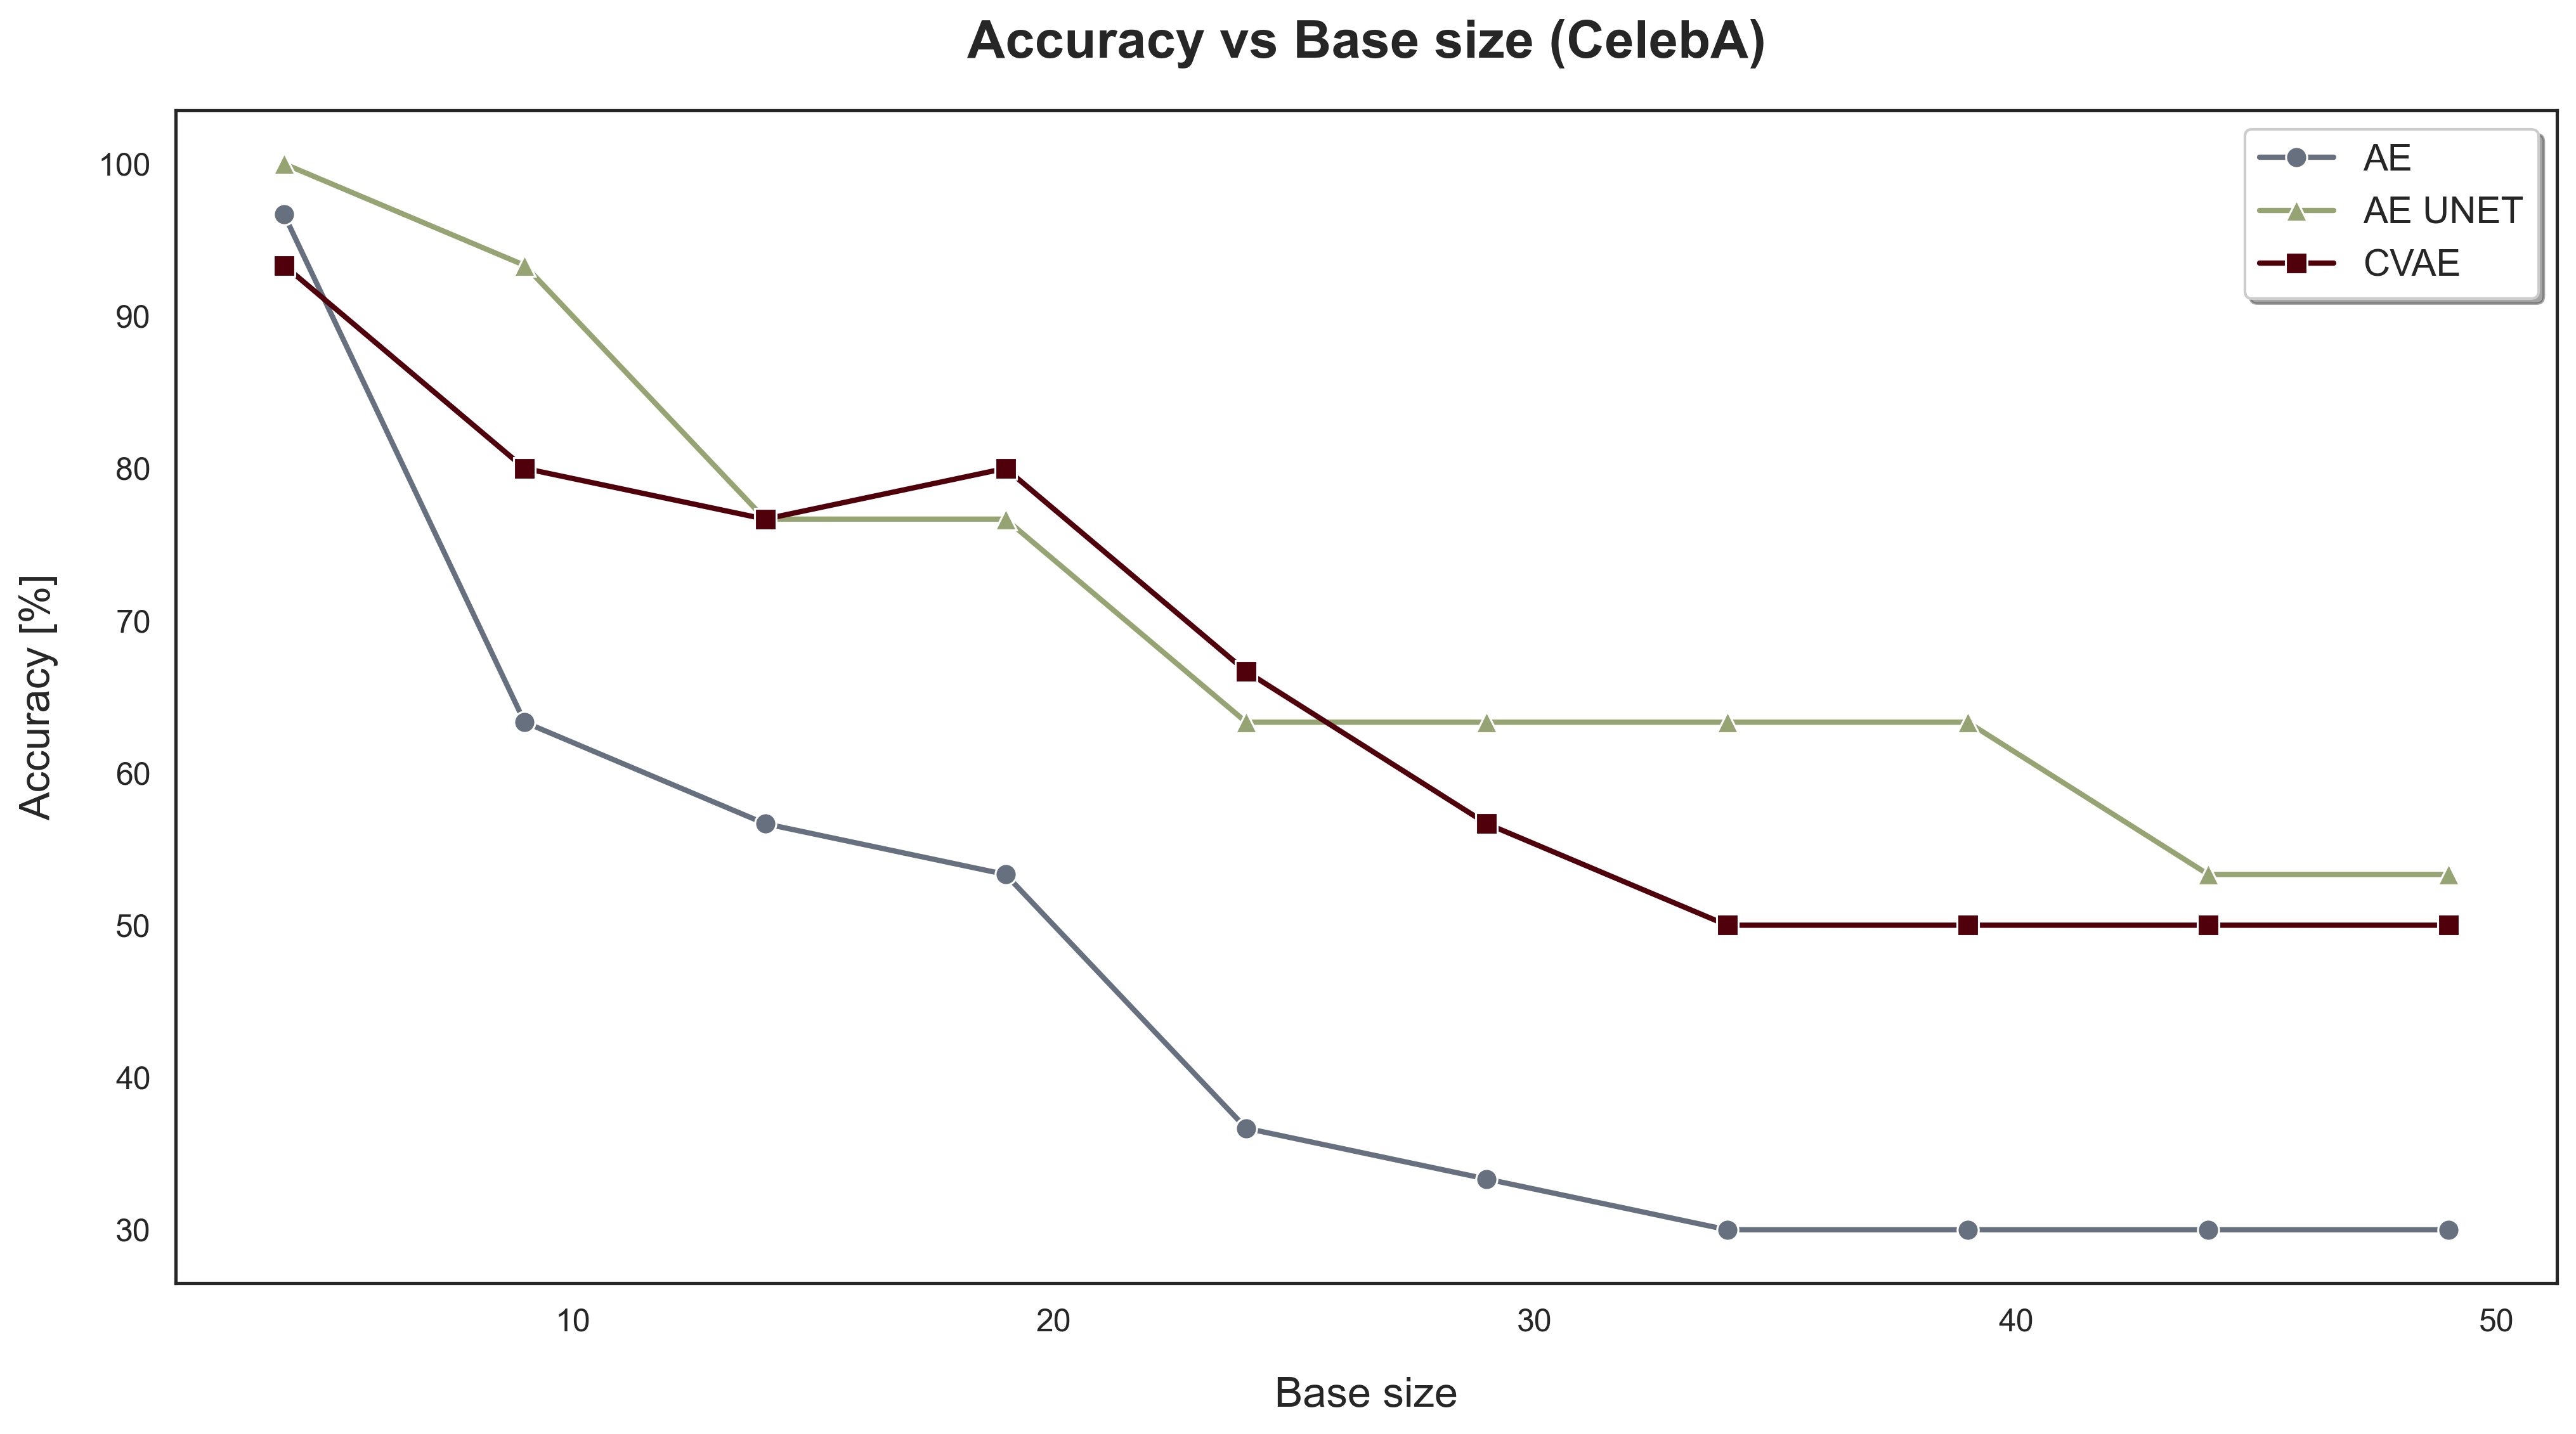
\includegraphics[width=\linewidth]{results/accuracy_vs_base_size_celeba.png}
        \caption{Accuracy of correct facial identification using CelebA.}
        \label{fig:accuracy_celeba}
    \end{subfigure}
    \hfill
    \begin{subfigure}{0.4\textwidth}
        \centering
        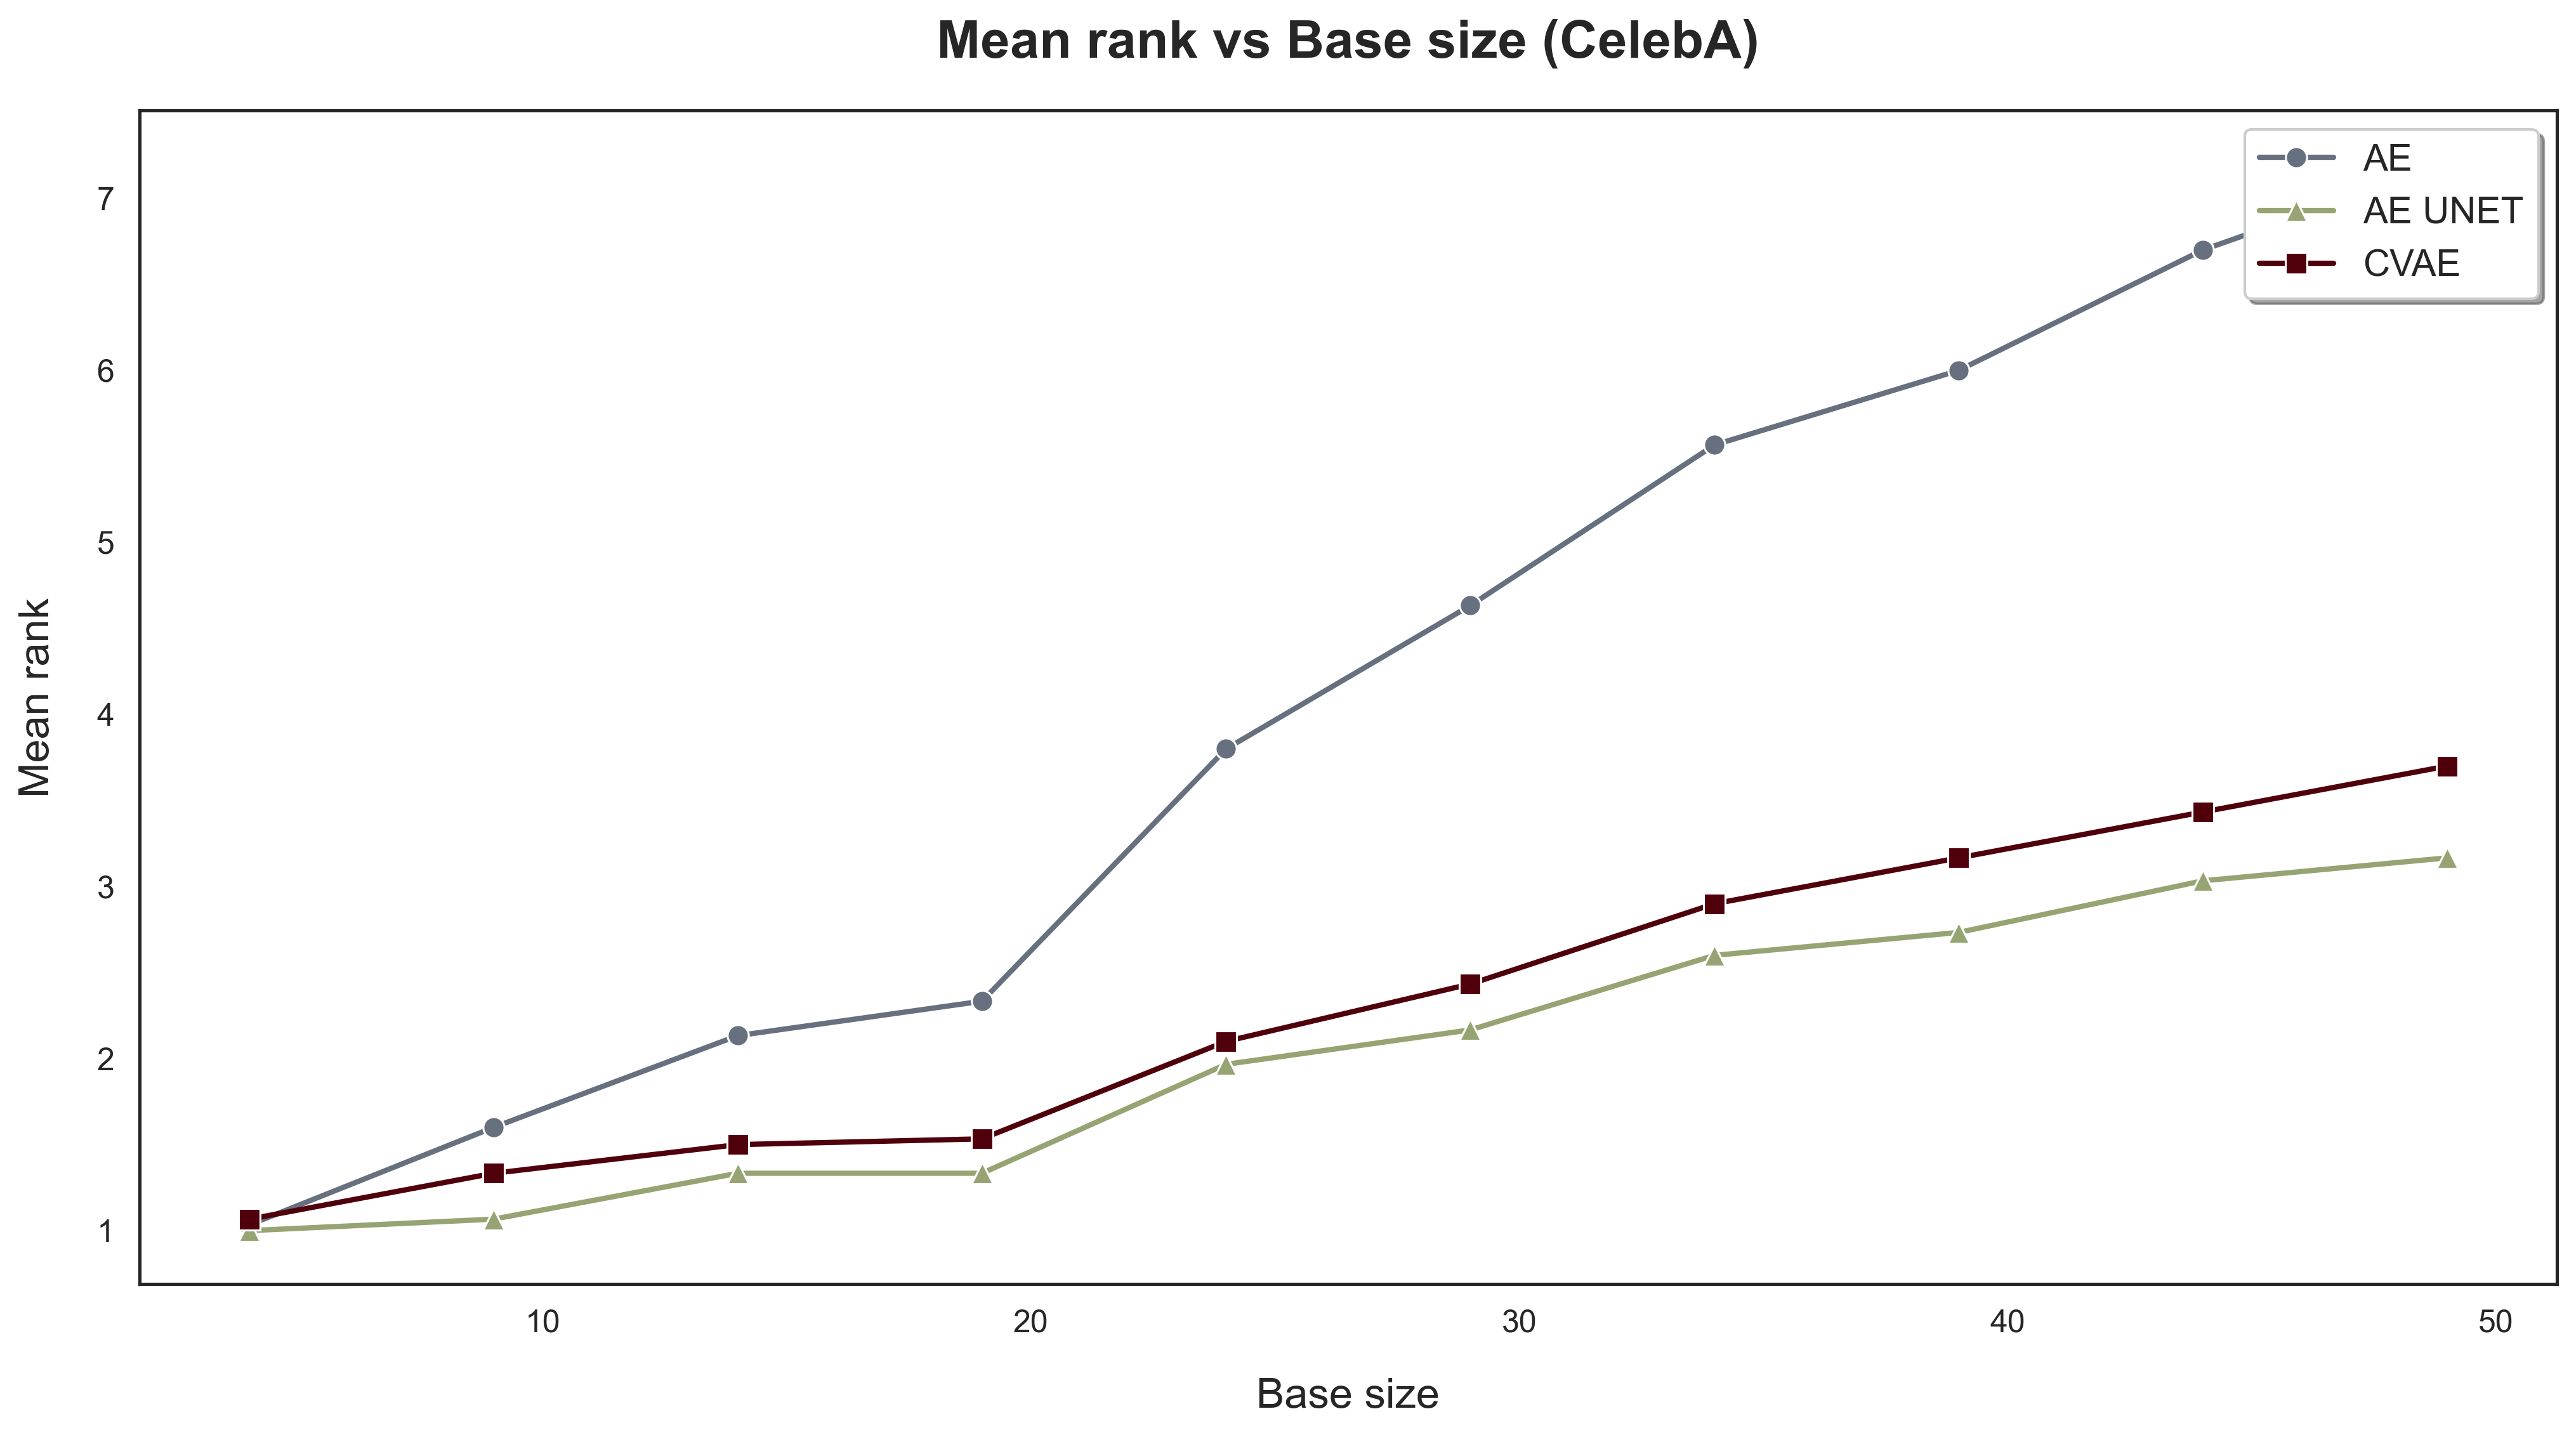
\includegraphics[width=\linewidth]{results/mean_vs_base_size_celeba.png}
        \caption{Mean rank of facial identification using CelebA.}
        \label{fig:mean_celeba}
    \end{subfigure}

    \begin{subfigure}{0.4\textwidth}
        \centering
        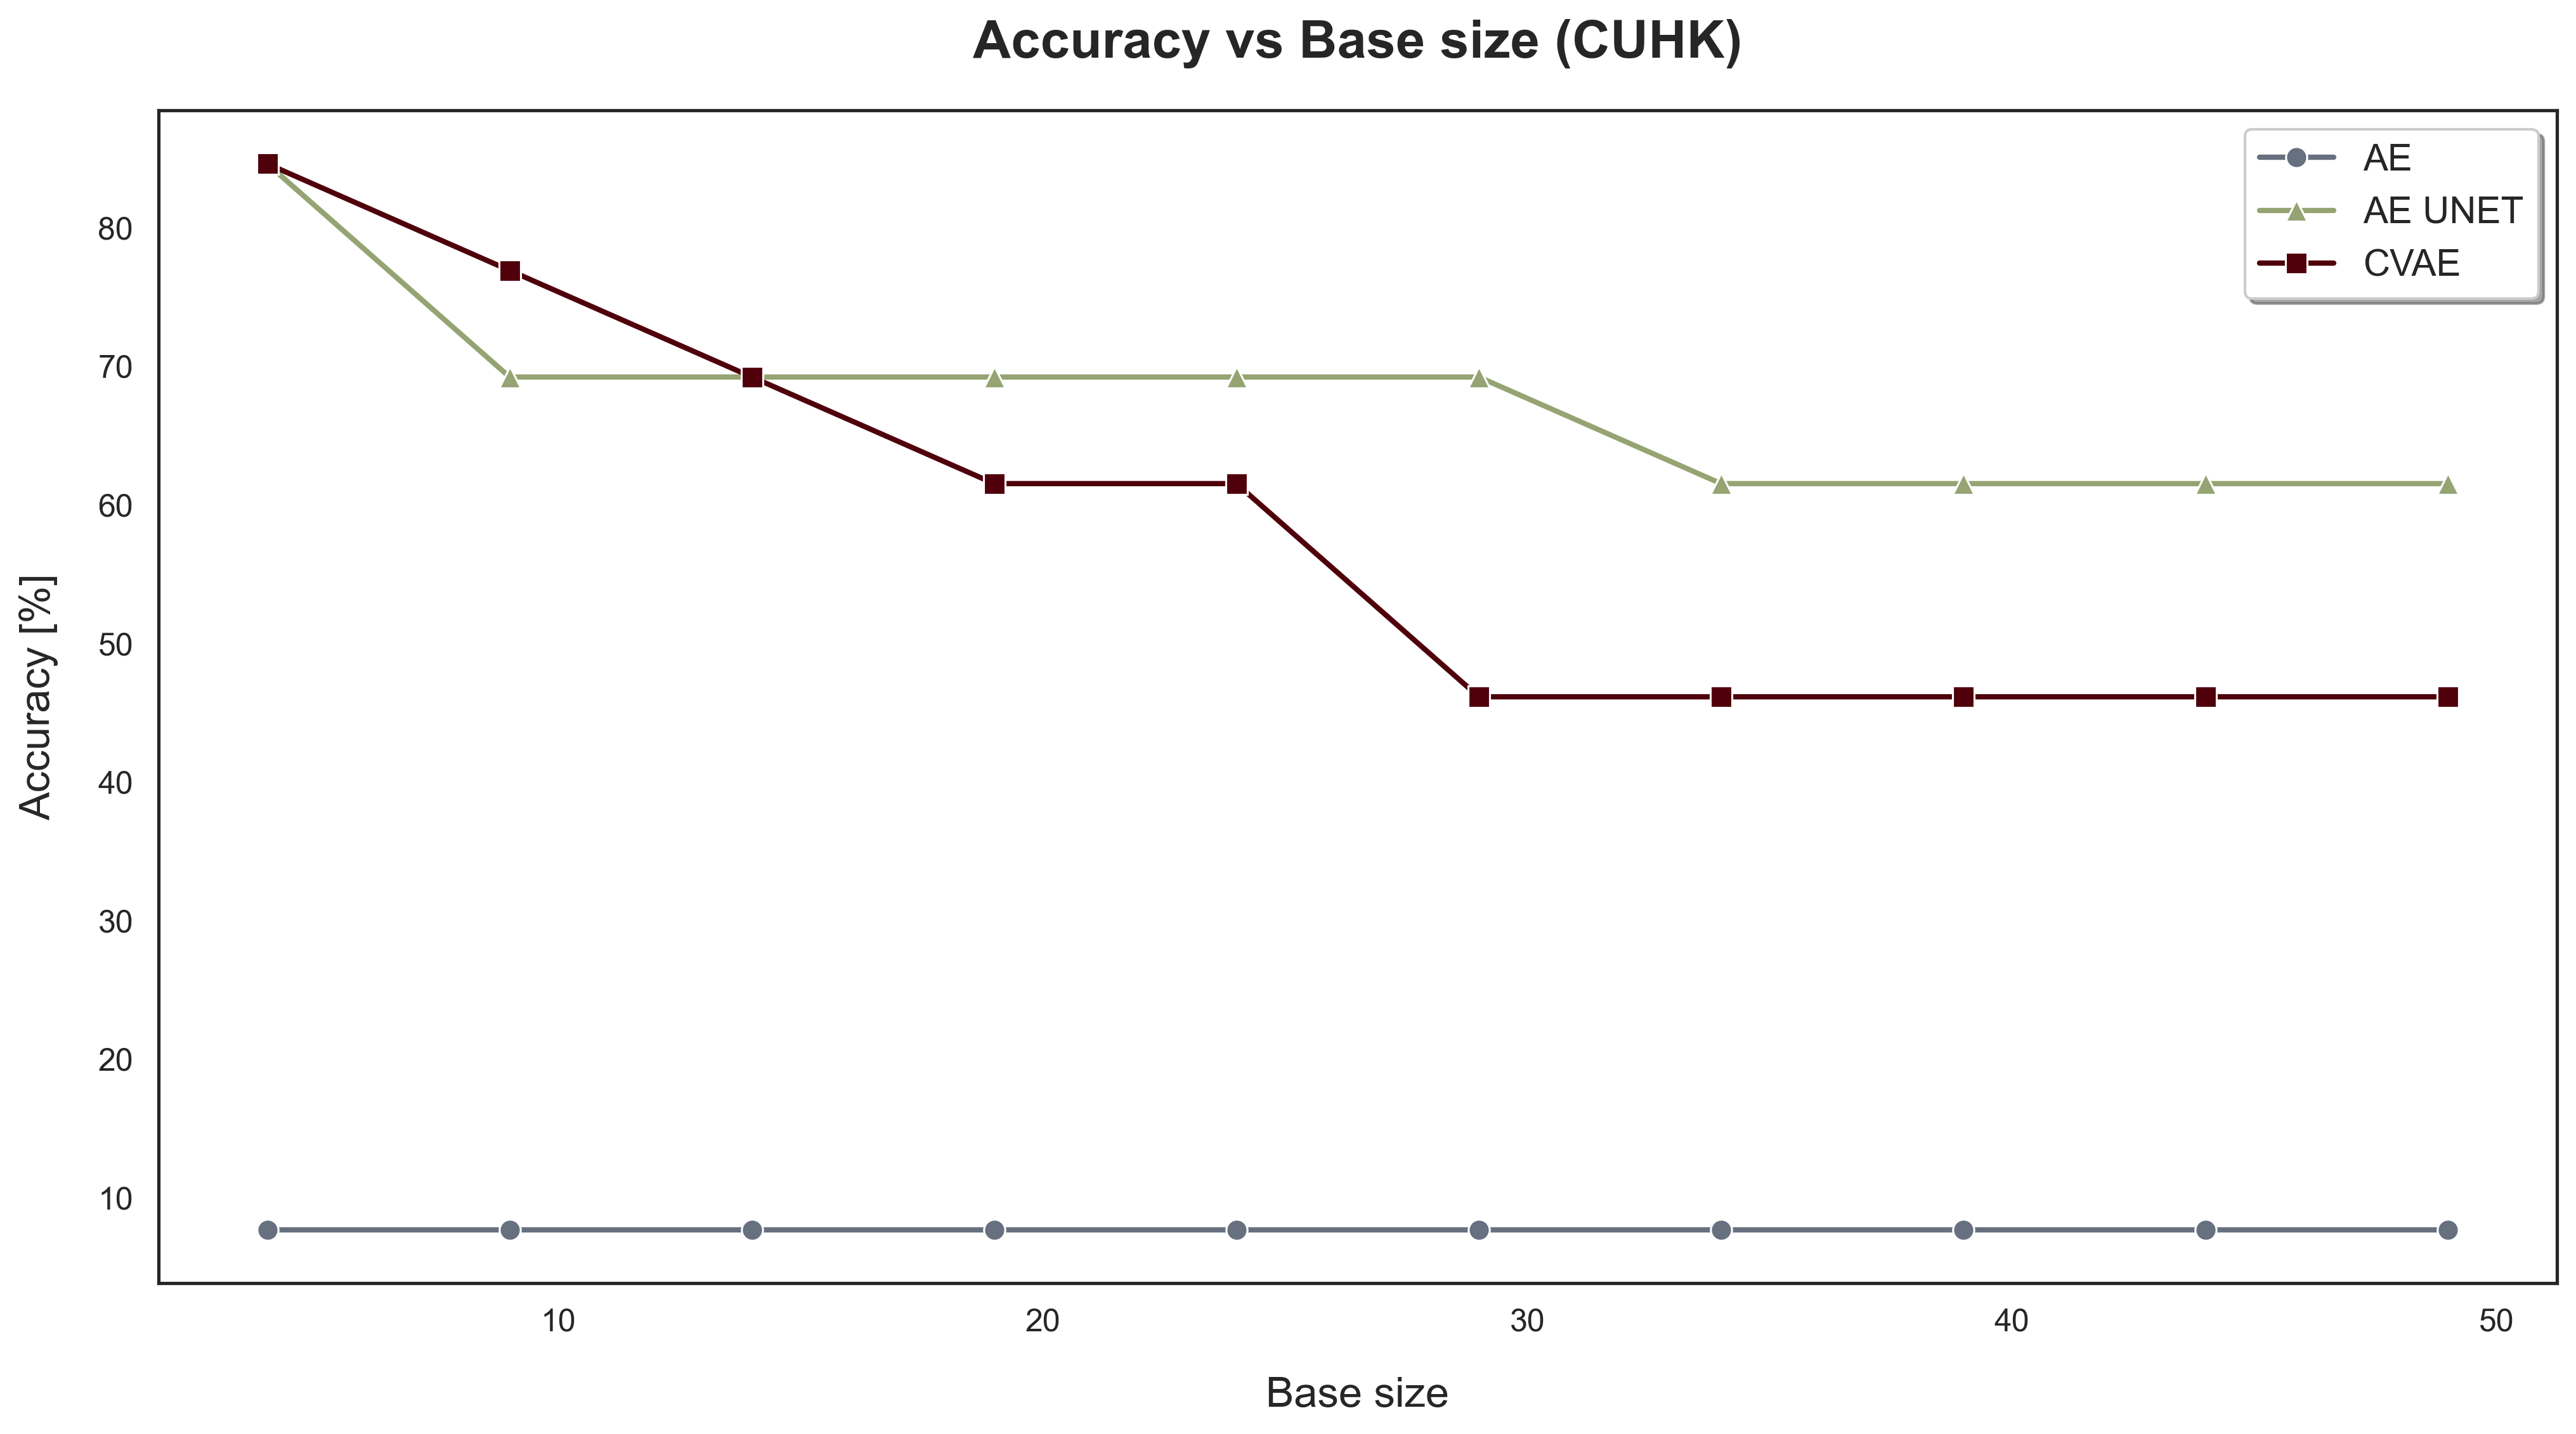
\includegraphics[width=\linewidth]{results/accuracy_vs_base_size_cuhk.png}
        \caption{Accuracy of correct facial identification using CUHK.}
        \label{fig:accuracy_cuhk}
    \end{subfigure}
    \hfill
    \begin{subfigure}{0.4\textwidth}
        \centering
        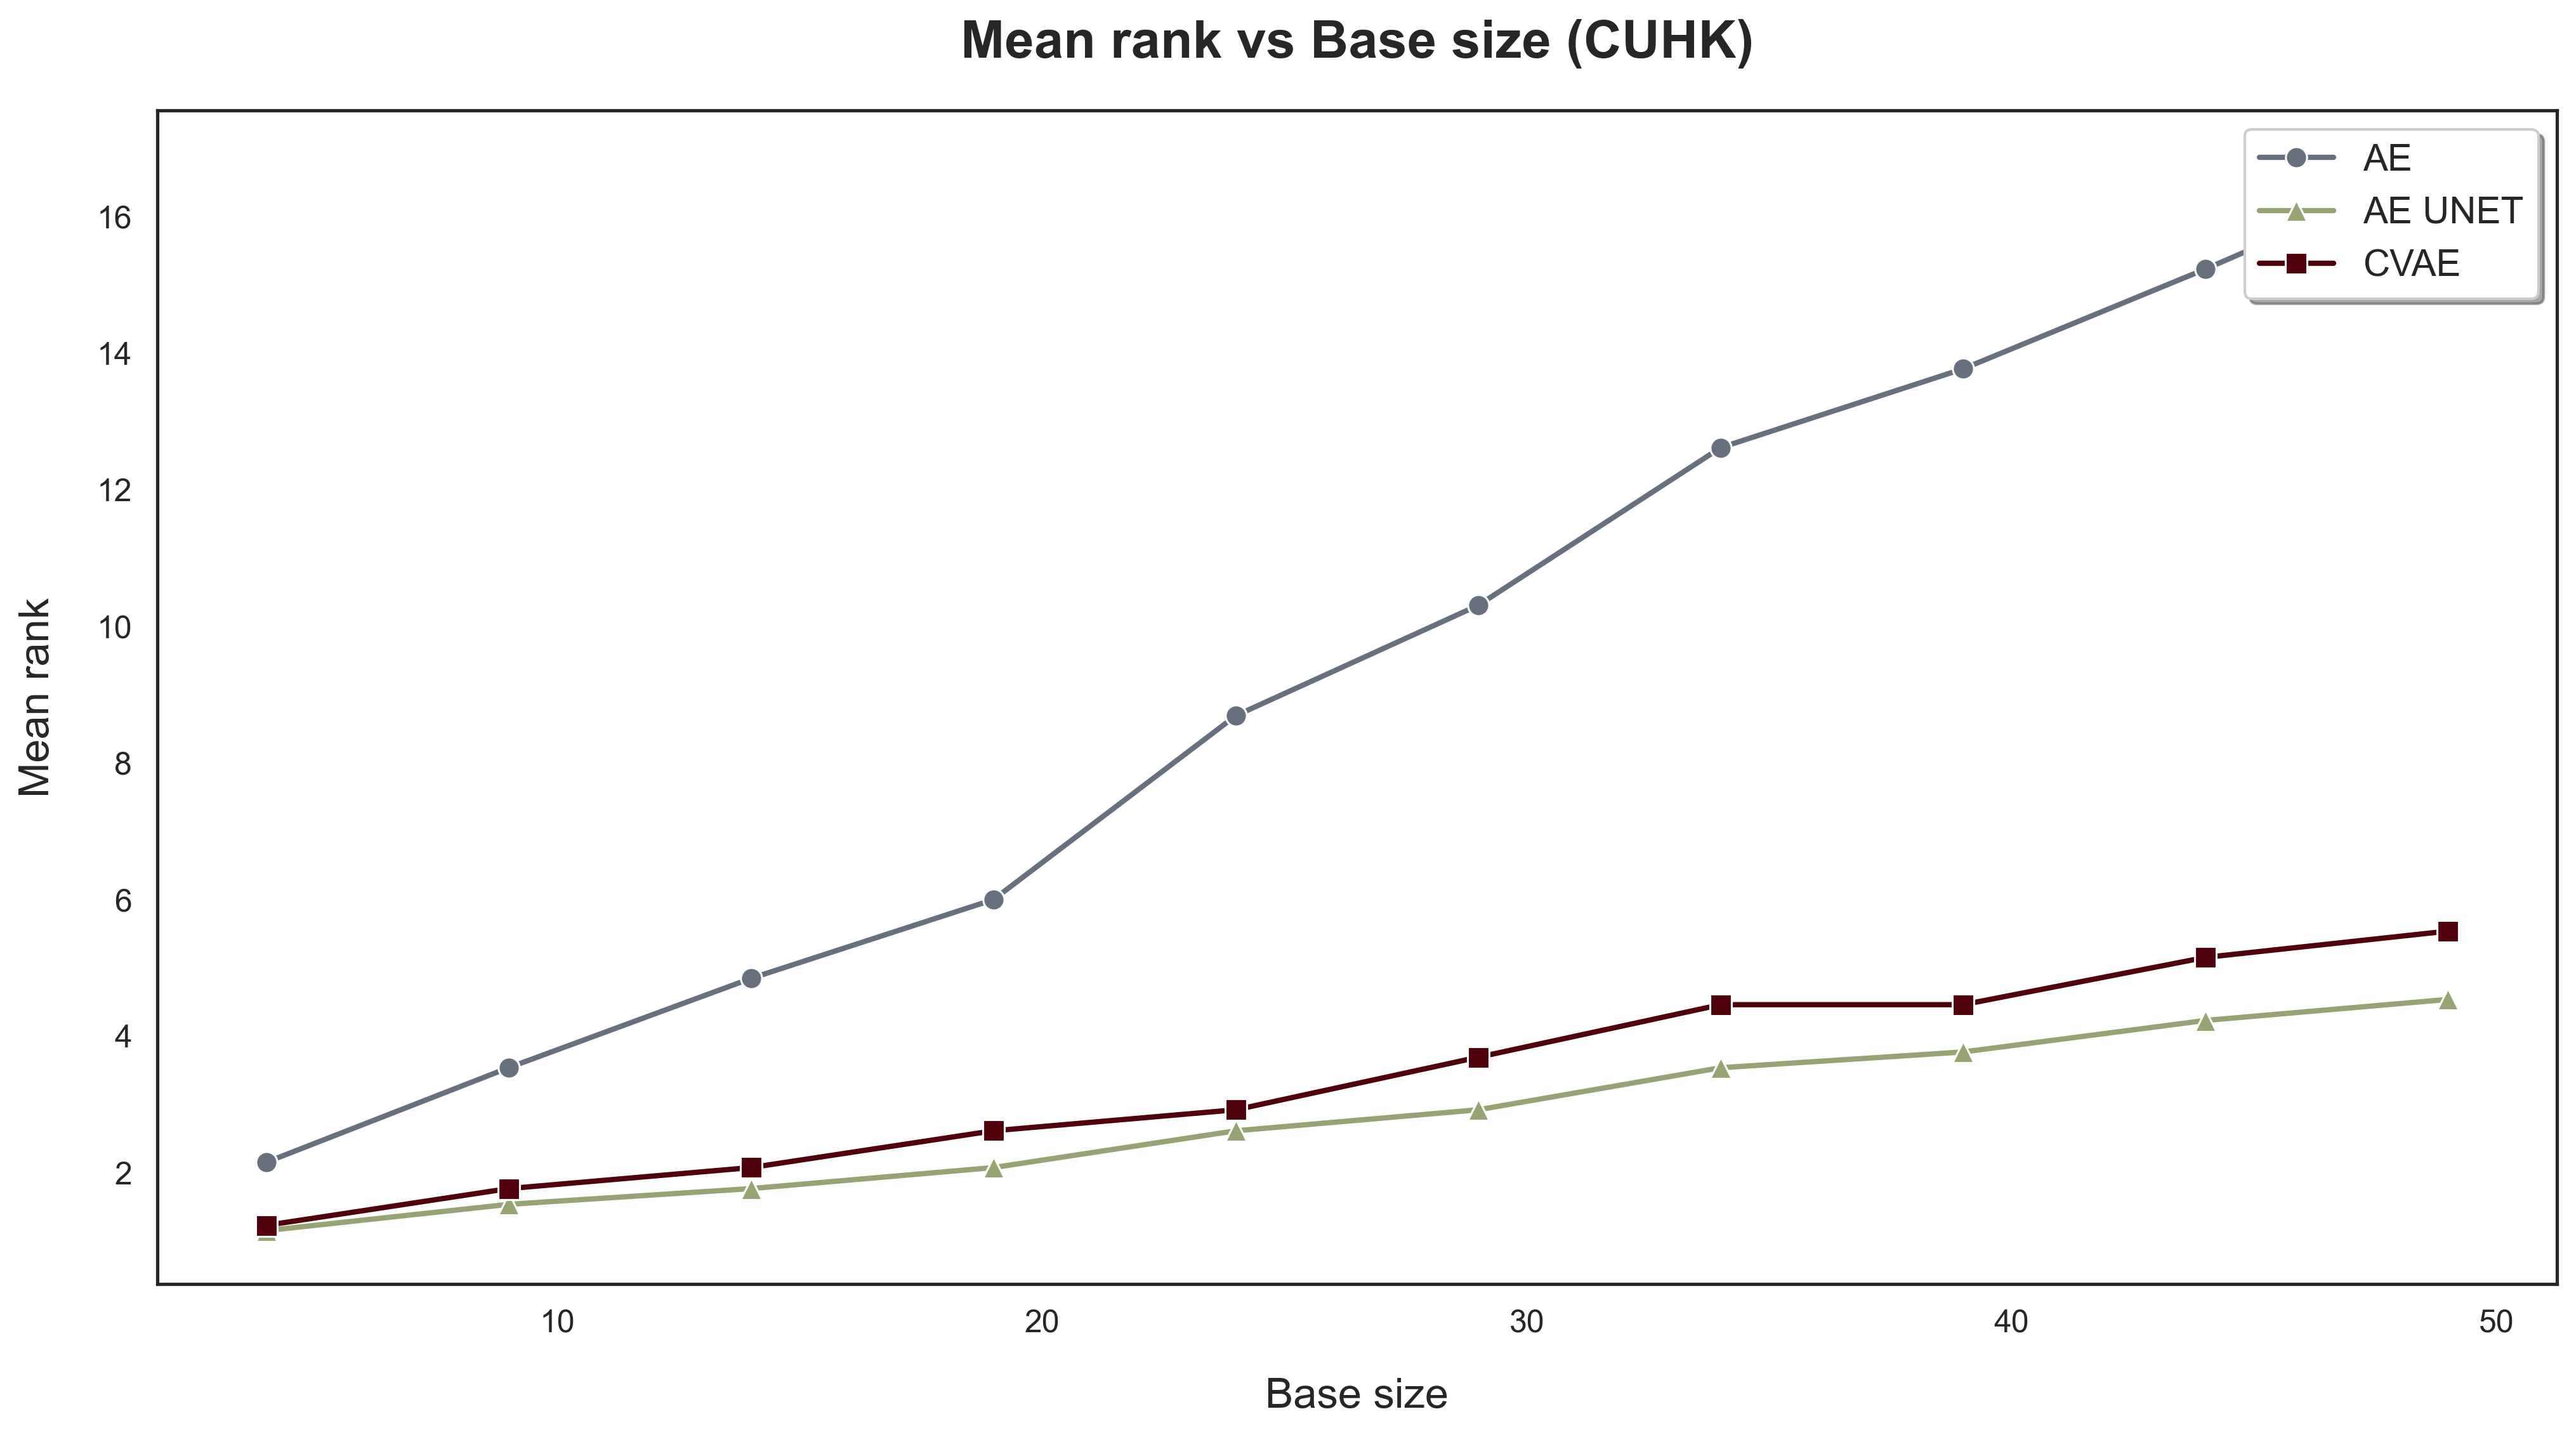
\includegraphics[width=\linewidth]{results/mean_vs_base_size_cuhk.png}
        \caption{Mean rank of facial identification using CUHK.}
        \label{fig:mean_cuhk}
    \end{subfigure}

    \caption{Comparison of facial identification performance using CelebA and CUHK datasets.}
    \label{fig:face_identification}
\end{figure*}

The performance of images that weren't correctly identified is explored. Figure \ref{fig:mean_celeba} shows the mean rank position of the suspects for each database size. Table \ref{tab:identification} shows that with 50 images of CelebA the mean rank of the vanilla AE is 7.2, roughly two times the mean rank of the proposed models. Figure \ref{fig:accuracy_cuhk} illustrates the accuracy as a function of the database size for the CUHK Student database. The vanilla AE failed to correctly identify almost every face (only one face was correctly identified), indicating overfitting of the model to the CelebA database. In contrast, the proposed AE achieved an accuracy of 62\% in the biggest database, while the CVAE model reached approximately 46\%.

The mean rank shown in Figure \ref{fig:mean_cuhk} is similar to the one observed in the CelebA evaluation. However, the vanilla AE performed even worse (16.77), while the proposed AE (4.54) and CVAE (5.54) were able to maintain consistent performance, as seen in table \ref{tab:identification}. Even though the proposed AE presented better identification results, it's important to address the advantages of using the CVAE in scenarios where the AE-generated image fails to capture specific features such as skin color, hair color, facial expressions, or gender. The identification performance is shown in table \ref{tab:identification}. Additionally, these findings reinforce that reconstruction accuracy alone does not guarantee strong identification performance.

\begin{table*}
\vspace*{4pt}
\caption{Identification performance for CelebA and CUHK datasets with varying dataset sizes}
\label{tab:identification}
\tablefont
\begin{tabular*}{\textwidth}{@{}l l l p{30pt}<{\centering} p{30pt}<{\centering} p{30pt}<{\centering} p{30pt}<{\centering} p{30pt}<{\centering} p{30pt}<{\centering}@{}}
\toprule
\textbf{Dataset} & 
\textbf{Model} & 
\textbf{Metric} & 
\textbf{5} & 
\textbf{10} & 
\textbf{20} & 
\textbf{30} & 
\textbf{40} & 
\textbf{50} \\
\colrule
\multirow{15}{*}{CelebA} 
& \multirow{5}{*}{Vanilla AE} & \rule{0pt}{10pt}Accuracy     & 0.97 & 0.63 & 0.53 & 0.33 & 0.30 & 0.30 \\[3pt]
&  & Correct Count & 29   & 19   & 16   & 10   & 9    & 9    \\[3pt]
&  & Mean Rank     & 1.03 & 1.60 & 2.33 & 4.63 & 6.00 & 7.20 \\[3pt]
&  & Max Rank      & 2    & 4    & 7    & 15   & 21   & 25   \\[3pt]
\cline{2-9}
& \multirow{5}{*}{Proposed AE} & \rule{0pt}{10pt}Accuracy     & 1.00 & 0.93 & 0.77 & 0.63 & 0.63 & 0.53 \\[3pt]
&  & Correct Count & 30   & 28   & 23   & 19   & 19   & 16   \\[3pt]
&  & Mean Rank     & 1.00 & 1.07 & 1.33 & 2.17 & 2.73 & 3.17 \\[3pt]
&  & Max Rank      & 1    & 2    & 4    & 7    & 11   & 14   \\[3pt]
\cline{2-9}
& \multirow{5}{*}{CVAE} & \rule{0pt}{10pt}Accuracy     & 0.93 & 0.80 & 0.80 & 0.57 & 0.50 & 0.50 \\[3pt]
&  & Correct Count & 28   & 24   & 24   & 17   & 15   & 15   \\[3pt]
&  & Mean Rank     & 1.07 & 1.33 & 1.53 & 2.43 & 3.17 & 3.70 \\[3pt]
&  & Max Rank      & 2    & 4    & 8    & 16   & 25   & 34   \\[3pt]
\colrule
\multirow{15}{*}{CUHK} 
& \multirow{5}{*}{Vanilla AE} & \rule{0pt}{10pt}Accuracy     & 0.08 & 0.08 & 0.08 & 0.08 & 0.08 & 0.08 \\[3pt]
&  & Correct Count & 1    & 1    & 1    & 1    & 1    & 1    \\[3pt]
&  & Mean Rank     & 2.15 & 3.54 & 6.00 & 10.31 & 13.77 & 16.77 \\[3pt]
&  & Max Rank      & 3    & 8    & 16   & 22   & 31   & 37   \\[3pt]
\cline{2-9}
& \multirow{5}{*}{Proposed AE} & \rule{0pt}{10pt}Accuracy     & 0.85 & 0.69 & 0.69 & 0.69 & 0.62 & 0.62 \\[3pt]
&  & Correct Count & 11   & 9    & 9    & 9    & 8    & 8    \\[3pt]
&  & Mean Rank     & 1.15 & 1.54 & 2.08 & 2.92 & 3.77 & 4.54 \\[3pt]
&  & Max Rank      & 2    & 4    & 7    & 13   & 18   & 21   \\[3pt]
\cline{2-9}
& \multirow{5}{*}{CVAE} & \rule{0pt}{10pt}Accuracy     & 0.85 & 0.77 & 0.62 & 0.46 & 0.46 & 0.46 \\[3pt]
&  & Correct Count & 11   & 10   & 8    & 6    & 6    & 6    \\[3pt]
&  & Mean Rank     & 1.23 & 1.77 & 2.62 & 3.69 & 4.46 & 5.54 \\[3pt]
&  & Max Rank      & 3    & 7    & 12   & 18   & 23   & 28   \\[3pt]
\botrule
\end{tabular*}
\vspace*{8pt}
\end{table*}

\subsection{Digital samples}
\label{subsec:digitalSamples}

The evaluation is extended to include digital sketches. Figure \ref{fig:DigitalSketchComparison} showcases faces generated from digitally drawn sketches. Some sketches are realistic, while others are more minimalistic. Despite these variations, the proposed models created images that captured some notable features of the faces depicted in the sketches.

The generated images are not flawless. For instance, sketch 2 resulted in a face with a distorted nose. This distortion can be attributed to the edge map detected in the nose area. Similarly, sketch 3 generated a face where the neck blends with the background. This issue arose because the sketch and its corresponding edge map did not clearly define the neck, leading to an ambiguous interpretation by the model.

\begin{figure*}[ht]
    \centering
    \setcounter{subfigure}{0}  % Reset subfigure counter
    
    % Row 1 - Sketch
    \begin{subfigure}{0.12\textwidth}
        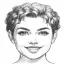
\includegraphics[width=\linewidth]{Prompted/draws_resized/image4.png}
        %\caption{Sketch 1}
    \end{subfigure}
    \begin{subfigure}{0.12\textwidth}
        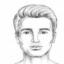
\includegraphics[width=\linewidth]{Digital sketches/draws_resized/image16.jpeg}
        %\caption{Sketch 2}
    \end{subfigure}
    \begin{subfigure}{0.12\textwidth}
        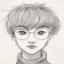
\includegraphics[width=\linewidth]{Digital sketches/draws_resized/image8.jpeg}
        %\caption{Sketch 3}
    \end{subfigure}
    \begin{subfigure}{0.12\textwidth}
        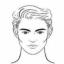
\includegraphics[width=\linewidth]{Digital sketches/draws_resized/image11.jpeg}
        %\caption{Sketch 4}
    \end{subfigure}
    \begin{subfigure}{0.12\textwidth}
        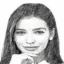
\includegraphics[width=\linewidth]{Random sketch/draws_resized/image2.jpeg}
        %\caption{Sketch 5}
    \end{subfigure}
    \begin{subfigure}{0.12\textwidth}
        
\includegraphics[width=\linewidth]{Digital sketches/draws_resized/image7.jpeg}
        %\caption{Sketch 6}
    \end{subfigure}

    \smallskip
    \setcounter{subfigure}{0}  % Reset subfigure counter
    
    % Row 2 - Edge Map
    \begin{subfigure}{0.12\textwidth}
        
\includegraphics[width=\linewidth]{Prompted/edge_map_resized/image4.png}
        %\caption{Edges 1}
    \end{subfigure}
    \begin{subfigure}{0.12\textwidth}
        
\includegraphics[width=\linewidth]{Digital sketches/edge_map_resized/image16.jpeg}
        %\caption{Edges 2}
    \end{subfigure}
    \begin{subfigure}{0.12\textwidth}
        
\includegraphics[width=\linewidth]{Digital sketches/edge_map_resized/image8.jpeg}
        %\caption{Edges 3}
    \end{subfigure}
    \begin{subfigure}{0.12\textwidth}
        
\includegraphics[width=\linewidth]{Digital sketches/edge_map_resized/image11.jpeg}
        %\caption{Edges 4}
    \end{subfigure}
    \begin{subfigure}{0.12\textwidth}
        
\includegraphics[width=\linewidth]{Random sketch/edge_map_resized/image2.jpeg}
        %\caption{Edges 5}
    \end{subfigure}
    \begin{subfigure}{0.12\textwidth}
        \includegraphics[width=\linewidth]{Digital sketches/edge_map_resized/image7.jpeg}
        %\caption{Edges 6}
    \end{subfigure}

    \smallskip
    \setcounter{subfigure}{0}  % Reset subfigure counter

    % Row 3 - Simple AE
    \begin{subfigure}{0.12\textwidth}
        \includegraphics[width=\linewidth]{Prompted/generated_images/image4.webp_AE.png}
        %\caption{Simple AE 1}
    \end{subfigure}
    \begin{subfigure}{0.12\textwidth}
        \includegraphics[width=\linewidth]{Digital sketches/generated_images/image16.jpeg_AE.png}
        %\caption{Simple AE 2}
    \end{subfigure}
    \begin{subfigure}{0.12\textwidth}
        \includegraphics[width=\linewidth]{Digital sketches/generated_images/image8.jpeg_AE.png}
        %\caption{Simple AE 3}
    \end{subfigure}
    \begin{subfigure}{0.12\textwidth}
        \includegraphics[width=\linewidth]{Digital sketches/generated_images/image11.jpeg_AE.png}
        %\caption{Simple AE 4}
    \end{subfigure}
    \begin{subfigure}{0.12\textwidth}
        \includegraphics[width=\linewidth]{Random sketch/generated_images/image2.jpeg_AE.png}
        %\caption{Simple AE 5}
    \end{subfigure}
    \begin{subfigure}{0.12\textwidth}
        \includegraphics[width=\linewidth]{Digital sketches/generated_images/image7.jpeg_AE.png}
        %\caption{Simple AE 6}
    \end{subfigure}

    \smallskip
    \setcounter{subfigure}{0}  % Reset subfigure counter
    
    % Row 4 - Proposed AE
    \begin{subfigure}{0.12\textwidth}
        \includegraphics[width=\linewidth]{Prompted/generated_images/image4.webp_AE_UNET.png}
        %\caption{Prop. AE 1}
    \end{subfigure}
    \begin{subfigure}{0.12\textwidth}
        \includegraphics[width=\linewidth]{Digital sketches/generated_images/image16.jpeg_AE_UNET.png}
        %\caption{Prop. AE 2}
    \end{subfigure}
    \begin{subfigure}{0.12\textwidth}
        \includegraphics[width=\linewidth]{Digital sketches/generated_images/image8.jpeg_AE_UNET.png}
        %\caption{Prop. AE 3}
    \end{subfigure}
    \begin{subfigure}{0.12\textwidth}
        \includegraphics[width=\linewidth]{Digital sketches/generated_images/image11.jpeg_AE_UNET.png}
        %\caption{Prop. AE 4}
    \end{subfigure}
    \begin{subfigure}{0.12\textwidth}
        \includegraphics[width=\linewidth]{Random sketch/generated_images/image2.jpeg_AE_UNET.png}
        %\caption{Prop. AE 5}
    \end{subfigure}
    \begin{subfigure}{0.12\textwidth}
        \includegraphics[width=\linewidth]{Digital sketches/generated_images/image7.jpeg_AE_UNET.png}
        %\caption{Prop. AE 6}
    \end{subfigure}

    \smallskip
    \setcounter{subfigure}{0}  % Reset subfigure counter

    % Row 5 - Proposed CVAE
    \begin{subfigure}{0.12\textwidth}
        \includegraphics[width=\linewidth]{Prompted/generated_images/image4.webp_CVAE.png}
        %\caption{Prop. CVAE 1}
    \end{subfigure}
    \begin{subfigure}{0.12\textwidth}
        \includegraphics[width=\linewidth]{Digital sketches/generated_images/image16.jpeg_CVAE.png}
        %\caption{Prop. CVAE 2}
    \end{subfigure}
    \begin{subfigure}{0.12\textwidth}
        \includegraphics[width=\linewidth]{Digital sketches/generated_images/image8.jpeg_CVAE.png}
        %\caption{Prop. CVAE 3}
    \end{subfigure}
    \begin{subfigure}{0.12\textwidth}
        \includegraphics[width=\linewidth]{Digital sketches/generated_images/image11.jpeg_CVAE.png}
        %\caption{Prop. CVAE 4}
    \end{subfigure}
    \begin{subfigure}{0.12\textwidth}
        \includegraphics[width=\linewidth]{Random sketch/generated_images/image2.jpeg_CVAE.png}
        %\caption{Prop. CVAE 5}
    \end{subfigure}
    \begin{subfigure}{0.12\textwidth}
        \includegraphics[width=\linewidth]{Digital sketches/generated_images/image7.jpeg_CVAE.png}
        %\caption{Prop. CVAE 6}
    \end{subfigure}

    \caption{Evaluation of Digital Sketches. Row 1: Original images; Row 2: Sketch or edge map; Row 3: Vanilla AE; Row 4: Proposed AE; Row 5: CVAE}
    \label{fig:DigitalSketchComparison}
\end{figure*}

\subsection{Conditional adjustments}
\label{subsec:conditionalAdjustments}

Figure \ref{fig:interpolation} illustrates the generated images created by interpolating the conditional inputs. The smiling attribute shown in the first sequence might be detectable from the sketch alone, while characteristics such as a pale face or blond hair in the second and third sequences are inferred by the model based on the provided conditions, reducing biases.

\begin{figure*}[ht]
    \centering
    \begin{subfigure}{0.8\textwidth}
        \includegraphics[width=\linewidth]{images/CelebA/5/Smiling/interpolation_13.png}
        %\caption{Smiling}
    \end{subfigure}
    \begin{subfigure}{0.8\textwidth}
        \includegraphics[width=\linewidth]{images/CelebA/5/Pale_Skin/interpolation_13.png}
        %\caption{Pale skin}
    \end{subfigure}
    \begin{subfigure}{0.8\textwidth}
        \includegraphics[width=\linewidth]{images/CelebA/5/Blond_Hair/interpolation_13.png}
        %\caption{Blond hair}
    \end{subfigure}
    \caption{Attribute interpolation across a range of values. The first image is the original, while the subsequent images show the effect of interpolating specific attributes from -2 to 2 in increments of 1. Row 1: Interpolate smiling; Row 2: Interpolate pale skin; Row 3: Interpolate blond hair.}
    \label{fig:interpolation}
\end{figure*}

These conditional inputs are more helpful when the model struggles to identify specific attributes based on the sketches. The flexibility provided by conditional adjustments allows for the exploration of different scenarios. Investigators can generate multiple variations of a suspect's image by adjusting conditions.

%\clearpage

\section{Conclusions}
\label{sec:conclusion}

This paper presented a novel CVAE architecture designed to generate photorealistic facial images from sketches and conditional attributes. The model was trained on artificial sketches and was rigorously evaluated using various styles of both digital and non-digital sketches. We also explored practical applications using a small database to define a list of suspects for identifying a generated suspect within this list. When evaluating with Facenet, the similarity using the CVAE is 56.8\% better than the vanilla AE, highlighting the strengths of the proposed models in generating facial images that are not only visually accurate but also recognizable using modern facial recognition models like Facenet. These models are expected to enhance forensic investigations, enabling quicker and more precise suspect identification, particularly when integrated with digital recognition systems.

For future research, we suggest increasing the image resolution and enhancing the preprocessing pipeline by incorporating additional techniques like extended difference-of-Gaussians (XDoG) or holistically-nested edge detection (HED) to create more refined edge maps. Additionally, integrating an adversarial loss could enhance image quality, provided it is applied carefully to preserve the essential features of the original image.

\bibliographystyle{IEEEtran}
\bibliography{reference} % Entries are in the refs.bib file

\end{document}

